\documentclass[a4paper,10pt]{book}
\usepackage{graphicx} 
\usepackage{geometry} 
\usepackage{fancyhdr} 
\usepackage{titlesec} 
\usepackage{multicol} 
\usepackage{float}
\usepackage{indentfirst}
\usepackage{pdfpages}

\geometry{top=0.25in, bottom=0.75in, left=0.75in, right=0.75in}

\pagestyle{fancy}
\fancyhf{}
\fancyfoot[C]{\thepage}

\titleformat{\chapter}[block]
  {\normalfont\Huge\bfseries}{\thechapter.}{0.5em}{\Huge}[\vspace{0.5cm}]

\title{\Huge \textbf{KOLA, CO NA OBIAD?}\\
\vspace{0.5cm}
\Large Skrypt dla studentów III roku Matematyki komputerowej}
\author{Autor: KOLA OWALSKA} 
\date{\vfill \large \textit{15 Października 2024}\\
\textit{New York, USA}}

\begin{document}
\maketitle
\newpage

\chapter*{Przedmowa} 
\thispagestyle{empty} 

Osobom postronnym często się wydaje, że badania matematyczne nie mają związku z otaczającą nas rzeczywistością. Jest to konsekwencja wysoce sformalizowanego języka, którym współczesnie posługuje się matematyka. Za tym formalizmem kryje się jednak bardzo bogaty świat matematycznych intuicji, bezpośrednio inspirowany nie tylko konkretnymi problemami nauki i techniki, ale przede wszystkim doświadczeniem i wyobrażeniami z codziennego życia. Matematycy rozwijają swoją intuicję wymyślając i analizując liczne przykłady. W przykładach tych poszukują powtarzających się prawidłowości. Jeśli taką prawidłowość uda się wykryć i nie udaje się znaleźć przykładu, w którym prawidłowość nie zachodzi, formułuje się hipotezę, że prawidłowość taka zachodzi zawsze. Hipoteza nie musi być i często nie jest w pełni prawidłowym opisem rzeczywistości, choć przynajmniej ziarno prawdy często w niej tkwi.

W odróżnieniu od wielu innych nauk, matematycy odrzucają intuicję i eksperyment jako metodę rozstrzygającą co jest prawdą. Hipotezę trzeba uzasadnić poprzez wyprowadzenie jej drogą logicznego rozumowania z uznawanych za oczywiste faktów. Rozumowanie takie nazywa się dowodem, a hipotezę, dla której udało się podać dowód, twierdzeniem. W tym miejscu pojawia się sformalizowany język. Przeprowadzenie matematycznego dowodu wymaga bowiem stosownej teorii. W teorii takiej ustala się najpierw podstawowe pojęcia, czyli tak zwane pojęcia pierwotne teorii oraz fakty uznawane za oczywiste, nazywane aksjomatami teorii. Wszystkie inne pojęcia teorii definiowane są w oparciu o pojęcia pierwotne, a twierdzenia dowodzone są w oparciu o przyjęte aksjomaty. Wysoki stopień sformalizowania języka matematycznego dowodu ma uniemożliwić, a przynajmniej utrudnić, świadome lub nieświadome przemycenie do dowodu fałszywego argumentu.

Tytuły przepisów po których następuje gwiazdka oznaczają dania wegetariańskie.

\vspace{1cm} 
\begin{flushright}
    \textit{"In these days the angel of topology and the devil of abstract algebra fight for the soul of every individual discipline of mathematics."} \\
    \textit{- Hermann Weyl}
\end{flushright}

\newpage 

\renewcommand{\contentsname}{Spis treści} 
\tableofcontents
\newpage

\chapter{Owsianka z owocami*}

\vspace{0.1cm}
\small
\begin{minipage}{0.45\textwidth}
    \noindent \textbf{Czas:} 10 minut\\
    \textbf{Poziom trudności:} łatwy 
\end{minipage}
\begin{minipage}{0.45\textwidth}
    \noindent \textbf{Ilość sprzątania:} minimalna\\
    \textbf{Wymagany mysi sprzęt:} -
\end{minipage}
\normalsize
\vspace{0.5cm}

\begin{multicols}{2}

\section*{Składniki:}
\begin{itemize}
    \item 3 kopiaste łyżki błyskawicznych płatków owsianych
    \item 1 szklanka mleka
    \item 1 płaska łyżka miodu/cukru
    \item 1 łyżeczka nasionek chia (opcjonalnie)
    \item 1 łyżeczka siemienia lnianego (opcjonalnie)
\end{itemize}

\columnbreak

\begin{figure}[H]
    \centering
    \fbox{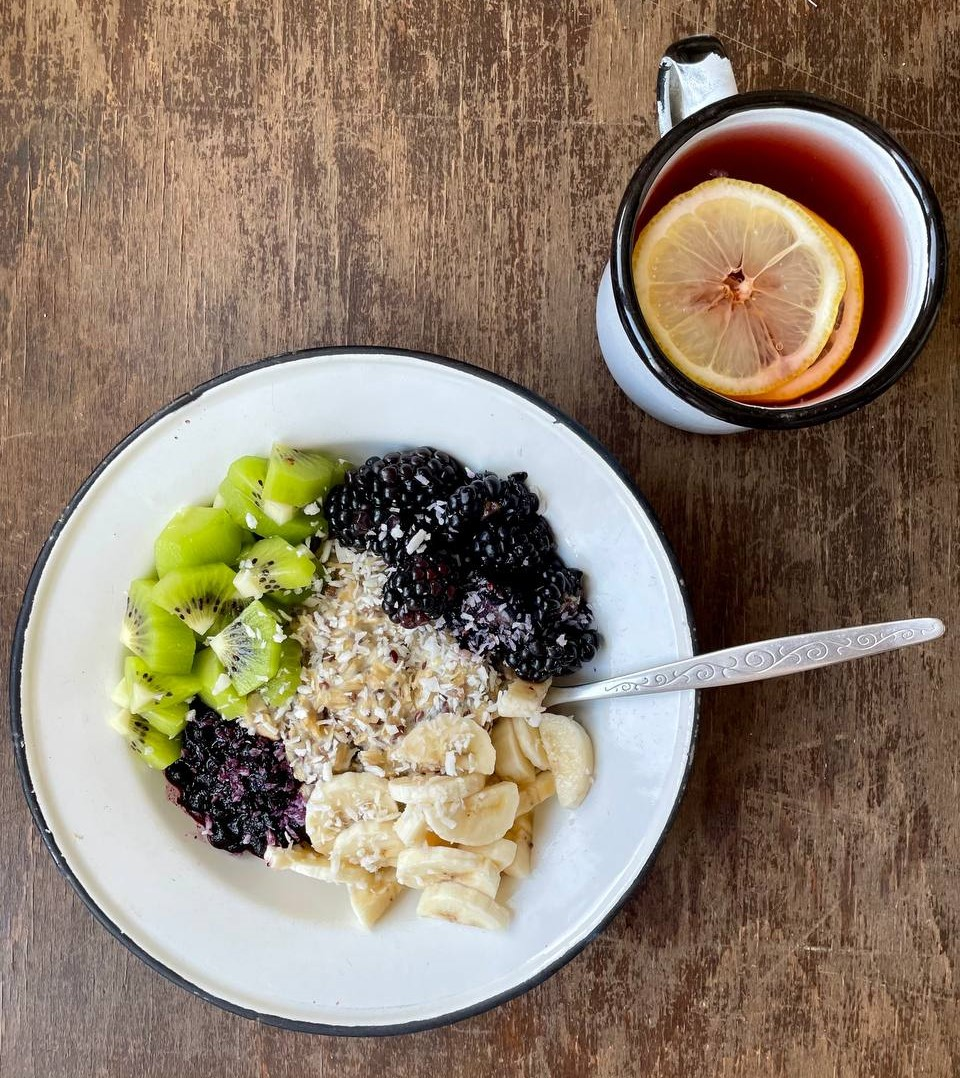
\includegraphics[width=0.35\textwidth]{images/owsianka.jpg}}
\end{figure}


\end{multicols}

\vspace{0.5cm} 

\section*{Instruktaż:}
\begin{enumerate}
    \item Płatki i nasiona wsypać do niewielkiego garnuszka, zalać mlekiem i mieszać od czasu do czasu aż mleko zacznie bulgotać.
    \item Gdy mleko osiągnie wysoką temperaturę, mieszać energicznie przez ok. 2 minuty.
\end{enumerate}

\vspace{0.5cm} 

\small
\section*{Propozycja podania:}
Z kawałkami czekolady, z jogurtem greckim, z owocami, z masłem orzechowym, z kremem czekoladowym, z wiórkami kokosowymi, z syropem klonowym

\vspace{0.3cm}

\section*{Dodatkowe uwagi:}
Owsiankę można urozmaicić smakowo poprzez dodanie do mleka cynamonu, przyprawy do piernika, kakao, masła orzechowego, płatków śniadaniowych, pokrojonego banana lub innych owoców, kawałków czekolady bądź orzechów (np. zimowa owsianka z jabłkami prażonymi i cynamonem, owsianka bakaliowa z kawałkami czekolady i orzechami, owsianka z bananem i masłem orzechowym)

\newpage 

% Recipe 2
\chapter{Tosty francuskie na słono*}

\vspace{0.1cm}
\small
\begin{minipage}{0.45\textwidth}
    \noindent \textbf{Czas:} 20 minut \\
    \textbf{Poziom trudności:} umiarkowany
\end{minipage}
\begin{minipage}{0.45\textwidth}
    \noindent \textbf{Ilość sprzątania:} średnia\\
    \textbf{Wymagany mysi sprzęt:} -
\end{minipage}
\normalsize
\vspace{0.5cm}

\begin{multicols}{2}

\section*{Składniki:}
\begin{itemize}
    \item 2 jajka z wolnego wybiegu
    \item 0.5 szklanki mleka
    \item 2 dojrzałe pomidory lub odpowiadająca ilość pomidorków koktajlowych
    \item 4 kromki (najlepiej czerstwego) chleba lub chleba tostowego
    \item oliwa do smażenia
    \item przyprawy
    \item sól i pieprz do smaku
\end{itemize}

\columnbreak

\begin{figure}[H]
    \centering
    \fbox{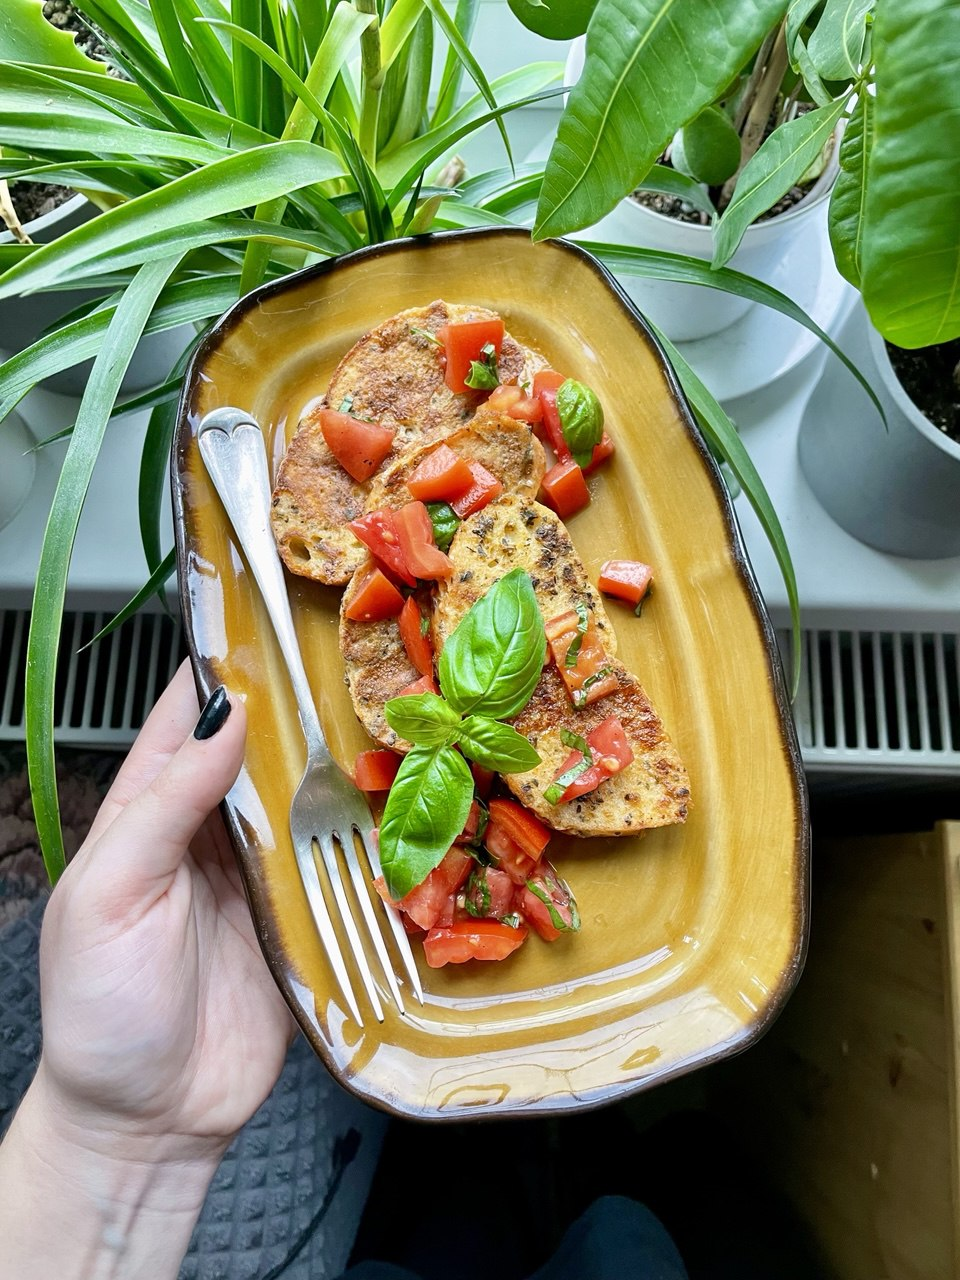
\includegraphics[width=0.35\textwidth]{images/tostynaslono.jpg}}
\end{figure}

\end{multicols}

\vspace{0.5cm} 

\section*{Instruktaż:}
\begin{enumerate}
    \item Pomidory pokroić w niewielką kostkę i przełożyć do miski. Doprawić odrobiną oliwy, płaską łyżeczką soli, pieprzu, majeranku, oregano, bazylii, tymianku, czosnku granulowanego. Wszystko dokładnie wymieszać i odstawić.
    \item Jajka roztrzepać z mlekiem i dodać po płaskiej łyżeczce soli, pieprzu i papryki słodkiej.
    \item Na rozgrzaną na średnim ogniu patelnię wlać oliwę i zaczekać, aż osiągnie temperaturę patelni. Kromki chleba pojedynczo lub parami namoczyć (ale nie rozmoczyć) w mieszance jajecznej z obu stron i smażyć na patelni z każdej strony, do momentu aż jajko się zetnie a tosty się zarumienią.
    \item Usmażone tosty przełożyć na talerz i serwować z krojonymi pomidorami.
\end{enumerate}

\vspace{0.5cm} 

\small
\section*{Propozycja podania:}
Z tartym serem, z listkami świeżej bazylii

\vspace{0.3cm}

\section*{Dodatkowe uwagi:}
Łatwo zamienić wytrawną wersję tostów na wersję na słodko - wystarczy mieszankę przypraw w miksturze jajecznej zastąpić niewielką ilością cukru i cynamonu, a zamiast z pomidorami serwować z dodatkami takimi jak jogurt, cukier puder, świeże owoce lub miód

\chapter{Naleśniczki bananowe*}

\vspace{0.1cm}
\small
\begin{minipage}{0.45\textwidth}
    \noindent \textbf{Czas:} 20 minut \\
    \textbf{Poziom trudności:} łatwy
\end{minipage}
\begin{minipage}{0.45\textwidth}
    \noindent \textbf{Ilość sprzątania:} średnia \\
    \textbf{Wymagany mysi sprzęt:} -
\end{minipage}
\normalsize
\vspace{0.5cm}

\begin{multicols}{2}

\section*{Składniki:} \begin{itemize} \item 2 dojrzałe banany \item 2 jajka \item 2 duże łyżki jogurtu greckiego \item 2 łyżki cukru lub miodu (opcjonalnie) \item szklanka mąki \item 2 łyżeczki proszku do pieczenia \item olej do smażenia \end{itemize}

\columnbreak

\begin{figure}[H] \centering 
\fbox{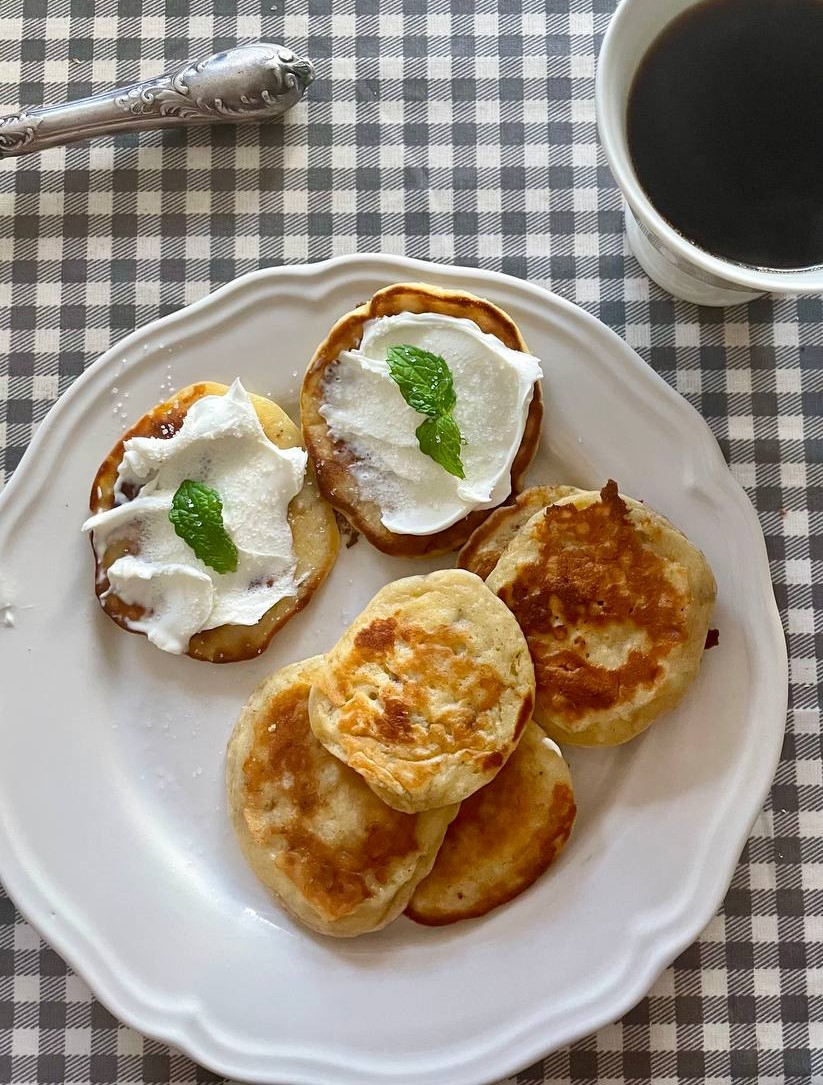
\includegraphics[width=0.35\textwidth]{images/nalesniczki.jpg}}
\end{figure}

\end{multicols}

\vspace{0.5cm}

\section*{Instruktaż:} \begin{enumerate} \item Banany rozgnieść widelcem na papkę, wbić jajka, ewentualnie dodać cukier, jogurt i wymieszać. \item Mąkę połączoną z proszkiem do pieczenia dodawać powoli i stopniowo, jednocześnie mieszając, aż do uzyskania jednolitej mikstury o odpowiedniej konsystencji. \item Patelnię rozgrzać na średnim ogniu, wlać niewielką ilość oleju i zaczekać około 2 minuty, aż nabierze temperatury. Zmniejszyć ogień i wlać po łyżce ciasta na każdego naleśniczka. Gdy krawędzie zaczną się ścinać lub pojawią się na nich bąbelki (około 3-5 minut), ostrożnie przewrócić na drugą stronę i smażyć, aż się zarumienią. \end{enumerate}

\vspace{0.5cm}

\small \section*{Propozycja podania:} Z bitą śmietaną, z cukrem pudrem, z dżemem, z jogurtem, z masłem orzechowym, z kremem czekoladowym, z owocami

\vspace{0.3cm}

\section*{Dodatkowe uwagi:} W zależności od tego, jak miękkie i dojrzałe są banany oraz jak duże są jajka, mieszanka może być zbyt wodnista lub zbyt gęsta - w takim wypadku należy dodać albo odrobinę więcej mąki, żeby ciasto zagęścić, albo niewielką ilość wody/mleka, aby stało się bardziej luźne.\ Ciasto można również urozmaicić poprzez dodanie do mąki odrobiny cynamonu, przyprawy do piernika, cukru wanilinowego lub kawałków czekolady

\chapter{Pasta jajeczna*}

\vspace{0.1cm}
\small
\begin{minipage}{0.45\textwidth}
    \noindent \textbf{Czas:} 10 minut \\
    \textbf{Poziom trudności:} łatwy
\end{minipage}
\begin{minipage}{0.45\textwidth}
    \noindent \textbf{Ilość sprzątania:} minimalna\\
    \textbf{Wymagany mysi sprzęt:} -
\end{minipage}
\normalsize
\vspace{0.5cm}

\begin{multicols}{2}

\section*{Składniki:}
\begin{itemize}
    \item 3 jajka z wolnego wybiegu
    \item 1 łyżka majonezu kieleckiego
    \item 1 mała cebula lub garstka drobno posiekanego szczypiorku/zielonej cebulki
    \item 100 g tartego sera (np. edamski lub gouda)
    \item sól i pieprz do smaku
\end{itemize}

\columnbreak

\begin{figure}[H]
    \centering
    \fbox{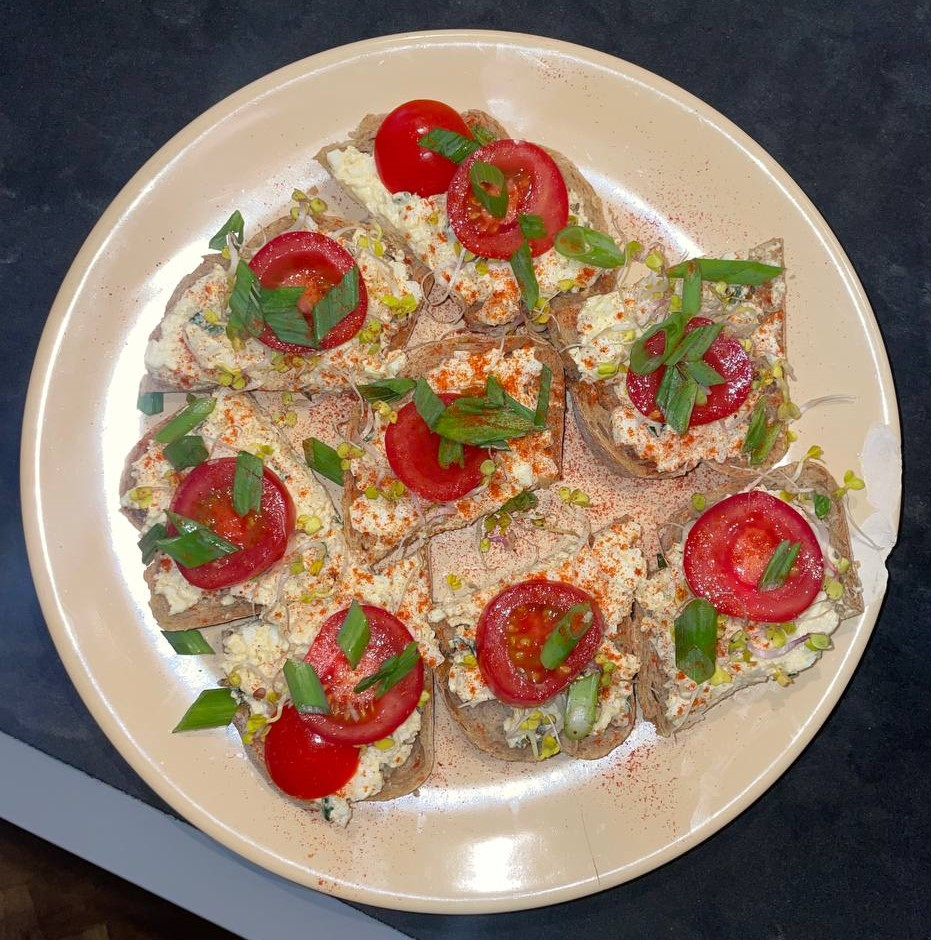
\includegraphics[width=0.35\textwidth]{images/pastajajeczna.jpg}}
\end{figure}
\end{multicols}

\vspace{0.5cm} 

\section*{Instruktaż:}
\begin{enumerate}
    \item Jajka ugotować na twardo. w międzyczasie posiekać cebulę na drobną kostkę i zetrzeć ser na tarce.
    \item Ostudzone jajka obrać ze skorupek, przełożyć do średniej wielkości miski i rozgniatać widelcem na drobne kawałki.
    \item Do miski z jajkami dodać pokrojoną cebulę, ser, majonez, szczyptę soli i pieprzu. wszystko dokładnie wymieszać i w razie potrzeby doprawić do smaku większą ilością soli i/lub pieprzu bądź większą ilością majonezu do uzyskania pożądanej konsystencji.
\end{enumerate}

\vspace{0.5cm} 

\small
\section*{Propozycja podania:}
Ze świeżym chlebem, z chrupiącą sałată, z plastrami pomidora lub ogórka, z papryką

\vspace{0.3cm}

\section*{Dodatkowe uwagi:}
Aby ostry smak surowej żółtej cebuli nie przytłaczał pozostałych składników, warto ją sparzyć - czyli posiekaną już w kawałki wrzucić do niewielkiej miseczki i zalać wrzątkiem na kilka minut. to spowoduje, że cebula w potrawach zachowa swój pyszny smak, a jednocześnie zaniknie jej nieprzyjemna ostrość

\chapter{Owoce pod kruszonką*}

\vspace{0.1cm}
\small
\begin{minipage}{0.45\textwidth}
    \noindent \textbf{Czas:} 60 minut \\
    \textbf{Poziom trudności:} łatwy
\end{minipage}
\begin{minipage}{0.45\textwidth}
    \noindent \textbf{Ilość sprzątania:} średnia\\
    \textbf{Wymagany mysi sprzęt:} -
\end{minipage}
\normalsize
\vspace{0.5cm}

\begin{multicols}{2}

\section*{Składniki:}
\begin{itemize}
    \item 250 g ulubionych owoców zważonych bez pestek (śliwki, jabłka, truskawki, czereśnie, brzoskwinie, gruszki, itp.)
    \item 1 łyżka miodu
    \item 1 płaska łyżka mąki ziemniaczanej
    \item 0.3(3) szklanki mąki (może być pszenna, pełnoziarnista, owsiana)
    \item 2 łyżki płatków owsianych 
    \item 2 łyżki cukru białego lub brązowego
    \item 0.25 kostki zimnego masła
    \item szczypta soli    
\end{itemize}

\columnbreak

\begin{figure}[H]
    \centering
    \fbox{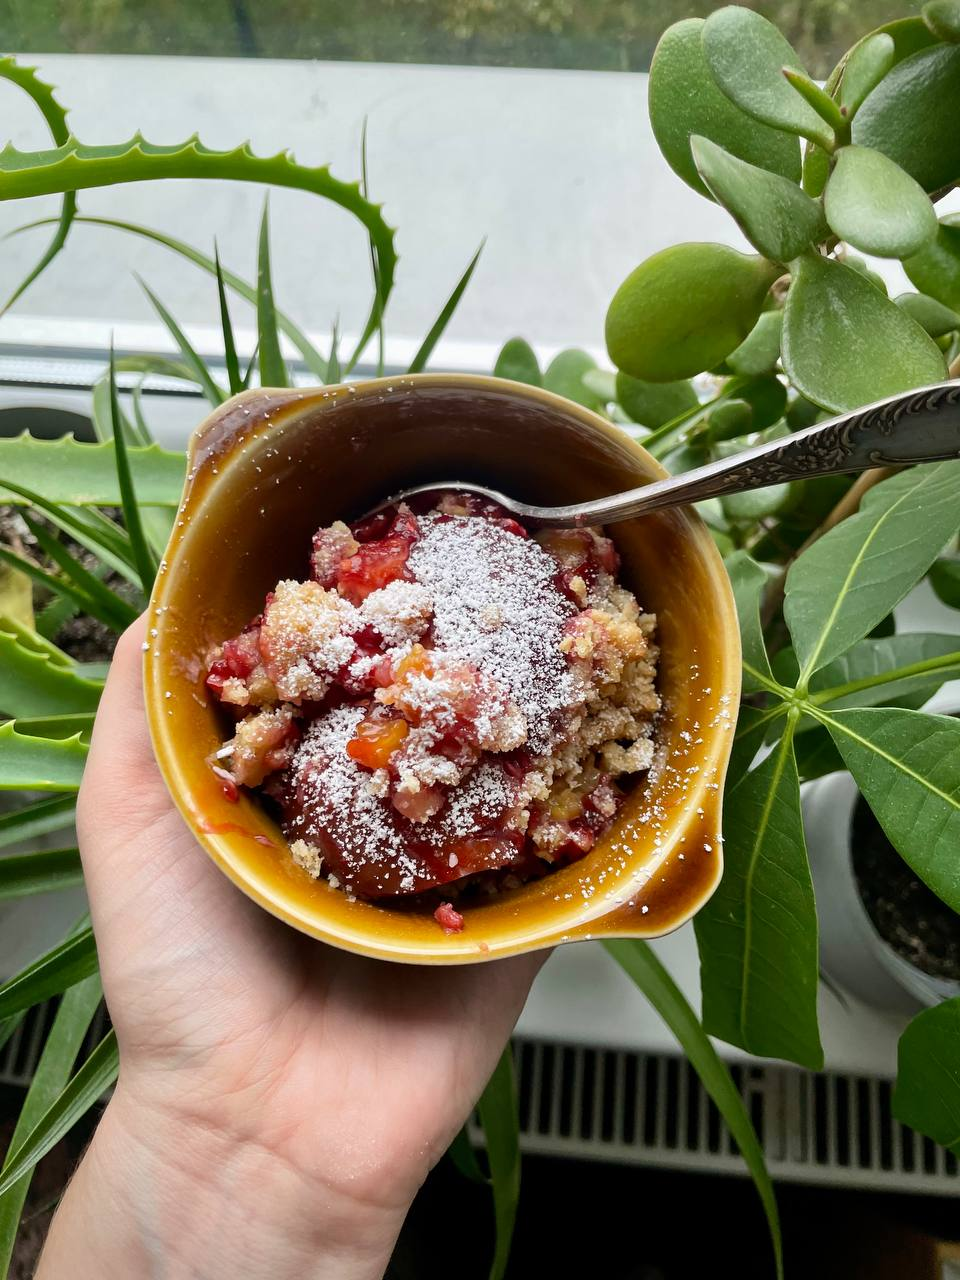
\includegraphics[width=0.35\textwidth]{images/kruszonka.jpg}}
\end{figure}
\end{multicols}

\vspace{0.5cm} 

\section*{Instruktaż:}
\begin{enumerate}
    \item Mąkę, płatki owsiane, szczyptę soli i cukier wymieszać dokładnie w misce i dodać masło pokrojone na małe kawałeczki. Rękami rozcierać masło razem z mąką, aż się połączą. Ciasto uformować w kulę, owinąć folią i wstawić do zamrażalnika na czas przygotowania owoców (10-15 minut).
    \item Piekarnik nagrzać do 180 stopni Celsjusza. Większe owoce jak brzoskwinie, śliwki, gruszki czy jabłka pokroić na kawałki przed włożeniem do naczynia żaroodpornego, polać miodem i posypać skrobią, po czym dokładnie wymieszać. 
    \item Kruszonkę wyjąć z zamrażalnika i pokruszyć palcami lub zetrzeć na tarce i posypać nią owoce.
    \item Całość piec około 40 minut, do momentu aż kruszonka się zarumieni, a sok owocowy zacznie bulgotać. 
\end{enumerate}

\vspace{0.5cm} 

\small
\section*{Propozycja podania:}
Z cukrem pudrem, z bitą śmietaną, z lodami, z jogurtem greckim

\vspace{0.3cm}

\section*{Dodatkowe uwagi:}
Nektarynki, brzoskwinie, czereśnie, borówki amerykańskie, maliny, truskawki, jeżyny, jagody, jabłka, gruszki, śliwki i morele – jeśli mrożone, należy piec 5 minut dłużej

\chapter{Zupa krem z pomidorów*}

\vspace{0.1cm}
\small
\begin{minipage}{0.45\textwidth}
    \noindent \textbf{Czas:} 60 minut \\
    \textbf{Poziom trudności:} łatwy
\end{minipage}
\begin{minipage}{0.45\textwidth}
    \noindent \textbf{Ilość sprzątania:} średnia\\
    \textbf{Wymagany mysi sprzęt:} duży garnek, blender
\end{minipage}
\normalsize
\vspace{0.5cm}

\begin{multicols}{2}

\section*{Składniki:}
\begin{itemize}
    \item 2 średniej wielkości marchewki
    \item 2 średniej wielkości korzenie pietruszki
    \item 2 cebule
    \item 4 duże ząbki czosnku
    \item 3 puszki pomidorów krojonych
    \item 1 opakowanie śmietany 18\%
    \item oliwa do smażenia
    \item 1 łyżka masła
    \item przyprawy
    \item kostka rosołowa (opcjonalnie)
    \item sól i pieprz do smaku
\end{itemize}

\columnbreak

\begin{figure}[H]
    \centering
    \fbox{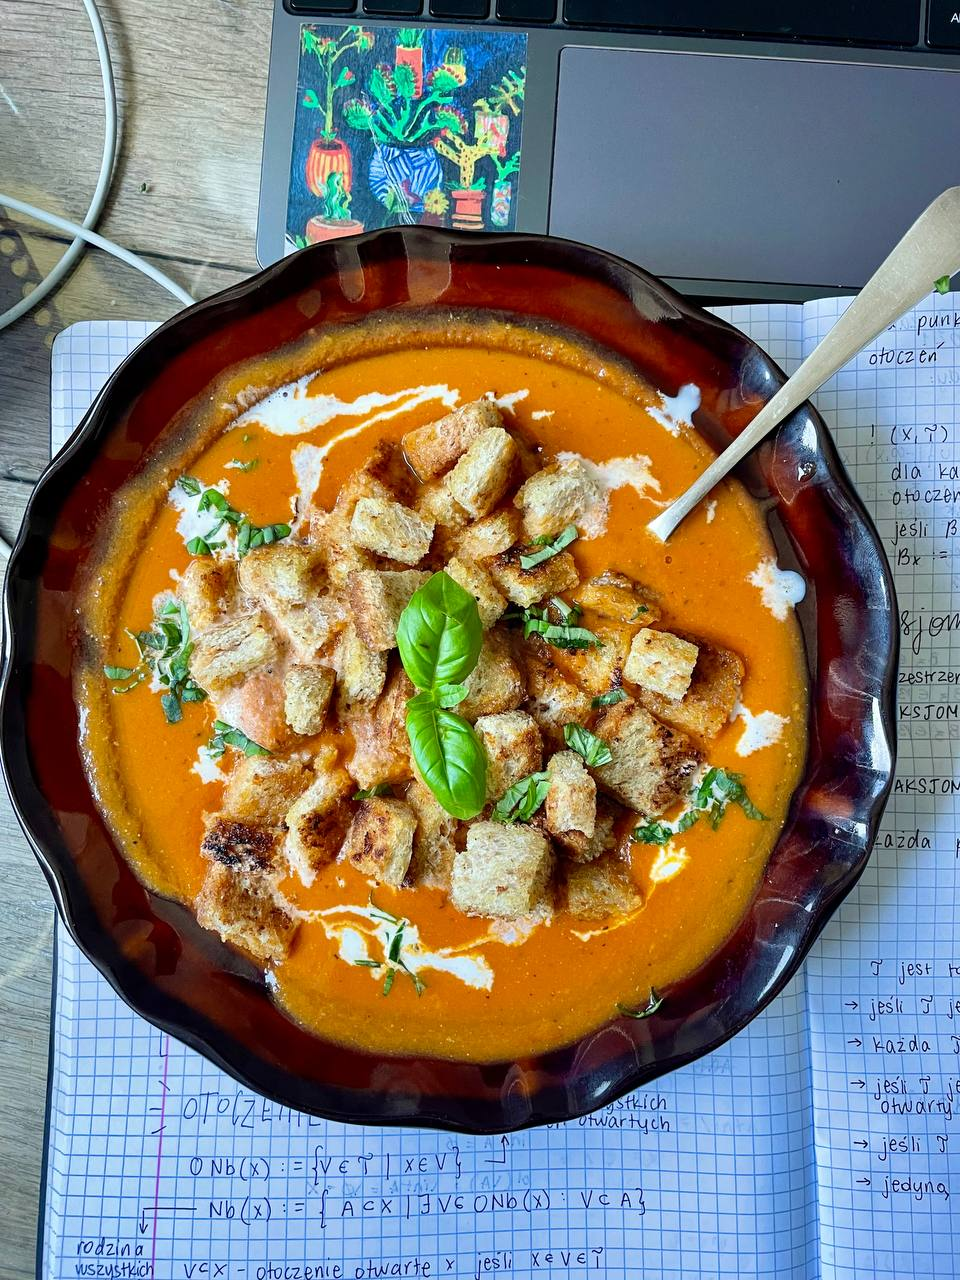
\includegraphics[width=0.35\textwidth]{images/pomidorowa.jpg}}
\end{figure}
\end{multicols}

\vspace{0.5cm} 

\section*{Instruktaż:}
\begin{enumerate}
    \item Pietruszkę oraz marchew obrać, przekroić wzdłuż na pół i pokroić na kawałki, po czym podsmażać na rozgrzanej oliwie i średnim ogniu przez około 5 minut (lub aż się zarumienią) od czasu do czasu mieszając. Dodać łyżeczkę soli, aby warzywa puściły wodę. W międzyczasie pokroić cebulę na średniej wielkości kostkę (nie musi być dokładna) i obrać czosnek.
    \item Po zarumienieniu się pietruszki i marchewki dosypać cebulę i podsmażać mieszając do momentu, aż cebula się zeszkli, czyli również około 5 minut. Warzywa posypać płaską łyżeczką kolejno: pieprzu, bazylii, majeranku, oregano, tymianku, rozmarynu i ewentualnie rozgniecioną kostkę rosołową. Wszystko dokładnie wymieszać. Obniżyć ogień na niski, warzywa na dnie garnka przesunąć na bok tak, aby się nie przypaliły.
    \item W wydzielone miejsce dodać masło i przeciśnięty przez praskę czosnek stale mieszając go w maśle tak, aby się nie przypalił, czyli około 20 sekund aż stanie się wonny. Po upływie 20 sekund wszystkie warzywa dokładnie wymieszać.
    \item Do garnka wlać pomidory. Każdą z puszek napełnić wodą w celu przepłukania ich i ją również wlać do garnka. Dodać łyżeczkę soli, wymieszać i gotować pod przykryciem na małym ogniu od czasu do czasu mieszając przez co najmniej 45 minut, aczkolwiek im dłużej, tym lepiej.
    \item Po skończonym gotowaniu ostudzić lekko zupę (można wystawić garnek na balkon w chłodną pogodę) i zblendować dokładnie. Śmietanę rozrobić z 2-3 łyżkami gorącej zupy i wlać do garnka. Dosolić do smaku.
\end{enumerate}

\vspace{0.5cm} 

\small
\section*{Propozycja podania:}
Z tościkiem z serem, z grzankami, z ryżem (żart), z listkami świeżej bazylii

\vspace{0.3cm}

\section*{Dodatkowe uwagi:}
Zupa świetnie się mrozi, dlatego też można bez problemu ugotować większą ilość, pozostawić do ostudzenia i przelać do pojemniczków, w których bezpiecznie się zamrozi - taki zapas awaryjny często przydaje się w dni, w które brakuje nam sił, aby ugotować obiad :)


\chapter{Zupa krem z cukinii*}

\vspace{0.1cm}
\small
\begin{minipage}{0.45\textwidth}
    \noindent \textbf{Czas:} 60 minut \\
    \textbf{Poziom trudności:} łatwy
\end{minipage}
\begin{minipage}{0.45\textwidth}
    \noindent \textbf{Ilość sprzątania:} średnia\\
    \textbf{Wymagany mysi sprzęt:} duży garnek, blender
\end{minipage}
\normalsize
\vspace{0.5cm}

\begin{multicols}{2}

\section*{Składniki:}
\begin{itemize}
    \item 2 średniej wielkości marchewki
    \item 2 średniej wielkości korzenie pietruszki
    \item 1 cebula
    \item 6 dużych ząbków czosnku
    \item 4 duże cukinie
    \item 1 opakowanie śmietany 18\%
    \item ok. 100 g sera z niebieską pleśnią (np. Lazur, Grand Blue)
    \item oliwa do smażenia
    \item 1 łyżka masła
    \item przyprawy
    \item kostka rosołowa (opcjonalnie)
    \item sól i pieprz do smaku
\end{itemize}

\columnbreak

\begin{figure}[H]
    \centering
    \fbox{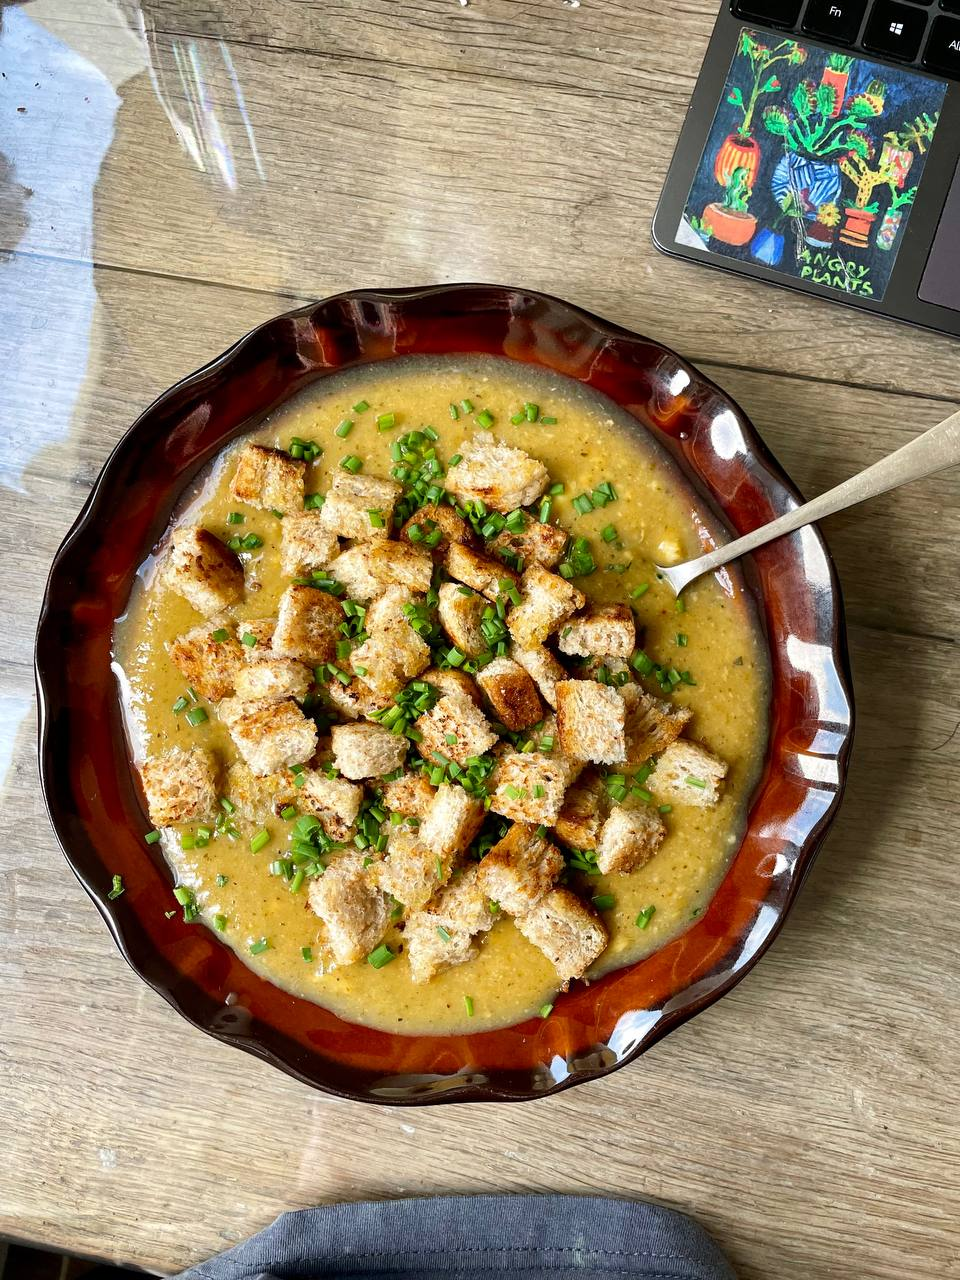
\includegraphics[width=0.4\textwidth]{images/cukiniowa.jpg}}
\end{figure}
\end{multicols}

\vspace{0.5cm} 

\section*{Instruktaż:}
\begin{enumerate}
    \item Cukinie dokładnie umyć i odkroić łodygę. Obieraczką do warzyw obierać każdą cukinię "w paski" , tzn. naprzemiennie na każdy obrany pasek pozostawić podobnej grubości pasek nieobranej skórki. Obrane cukinie przekroić wzdłuż na połowy, po czym każdą połowę przekroić ponownie wzdłuż. Jeśli pestek cukinii wewnątrz ćwiartek będzie zbyt wiele lub pojedyncze pestki będą łatwo widoczne, wyciąć nożem miąższ z nadmiarem pestek. Obrane i oczyszczone kawałki cukinii pokroić na duże kostki i odstawić na bok.
    \item Pietruszkę oraz marchew obrać, przekroić wzdłuż na pół i pokroić na kawałki, po czym podsmażać na rozgrzanej oliwie i średnim ogniu przez około 5 minut (lub aż się zarumienią) od czasu do czasu mieszając. Dodać łyżeczkę soli, aby warzywa puściły wodę. W międzyczasie pokroić cebulę na średniej wielkości kostkę (nie musi być dokładna) i obrać czosnek.
    \item Po zarumienieniu się pietruszki i marchewki dosypać cebulę i podsmażać mieszając do momentu, aż cebula się zeszkli, czyli również około 5 minut. Warzywa posypać płaską łyżeczką kolejno: pieprzu, bazylii, majeranku, tymianku, rozmarynu i ewentualnie rozgniecioną kostkę rosołową. Wszystko dokładnie wymieszać. Obniżyć ogień na niski, warzywa na dnie garnka przesunąć na bok tak, aby się nie przypaliły.
    \item W wydzielone miejsce dodać masło i przeciśnięty przez praskę czosnek stale mieszając go w maśle tak, aby się nie przypalił, czyli około 20 sekund aż stanie się wonny. Po upływie 20 sekund wszystkie warzywa dokładnie wymieszać.
    \item Do garnka dodać pokrojoną cukinię i dokładnie wymieszać z warzywami znajdującymi się na dnie garnka. Całość zalać taką ilością wrzątku, aby wszystkie warzywa były zanurzone. Dodać łyżeczkę soli, wymieszać i gotować pod przykryciem na małym ogniu od czasu do czasu mieszając przez co najmniej 45 minut, aczkolwiek im dłużej, tym lepiej.
    \item Po skończonym gotowaniu ostudzić lekko zupę (można wystawić garnek na balkon w chłodną pogodę) i zblendować dokładnie. Śmietanę rozrobić z 2-3 łyżkami gorącej zupy i wlać do garnka. Dosolić do smaku i w razie potrzeby, gdyby zupa była zbyt gęsta, dolać odrobinę wody, aby uzyskać pożądaną konsystencję. 
\end{enumerate}

\vspace{0.5cm} 

\small
\section*{Propozycja podania:}
Z domowymi grzankami, z chrupiącym tostem, ze startym długodojrzewającym serem, ze świeżymi ziołami

\vspace{0.3cm}

\section*{Dodatkowe uwagi:}
Zupa świetnie się mrozi, dlatego też można bez problemu ugotować większą ilość, pozostawić do ostudzenia i przelać do pojemniczków, w których bezpiecznie się zamrozi - taki zapas awaryjny często przydaje się w dni, w które brakuje nam sił, aby ugotować obiad :)


\chapter{Makaron z łososiem i warzywami}

\vspace{0.1cm}
\small
\begin{minipage}{0.45\textwidth}
    \noindent \textbf{Czas:} 20 minut \\
    \textbf{Poziom trudności:} umiarkowany
\end{minipage}
\begin{minipage}{0.45\textwidth}
    \noindent \textbf{Ilość sprzątania:} średnia\\
    \textbf{Wymagany mysi sprzęt:} -
\end{minipage}
\normalsize
\vspace{0.5cm}

\begin{multicols}{2}

\section*{Składniki:} \begin{itemize} 
\item 50-100 g wędzonego łososia 
\item 2 ząbki czosnku 
\item porcja makaronu 
\item 2 garści młodego szpinaku
\item garść pomidorków koktajlowych
\item 50 g śmietanki 18% 
\item oliwa do smażenia 
\item sól i pieprz do smaku
\end{itemize}

\columnbreak

\begin{figure}[H]
    \centering
    \fbox{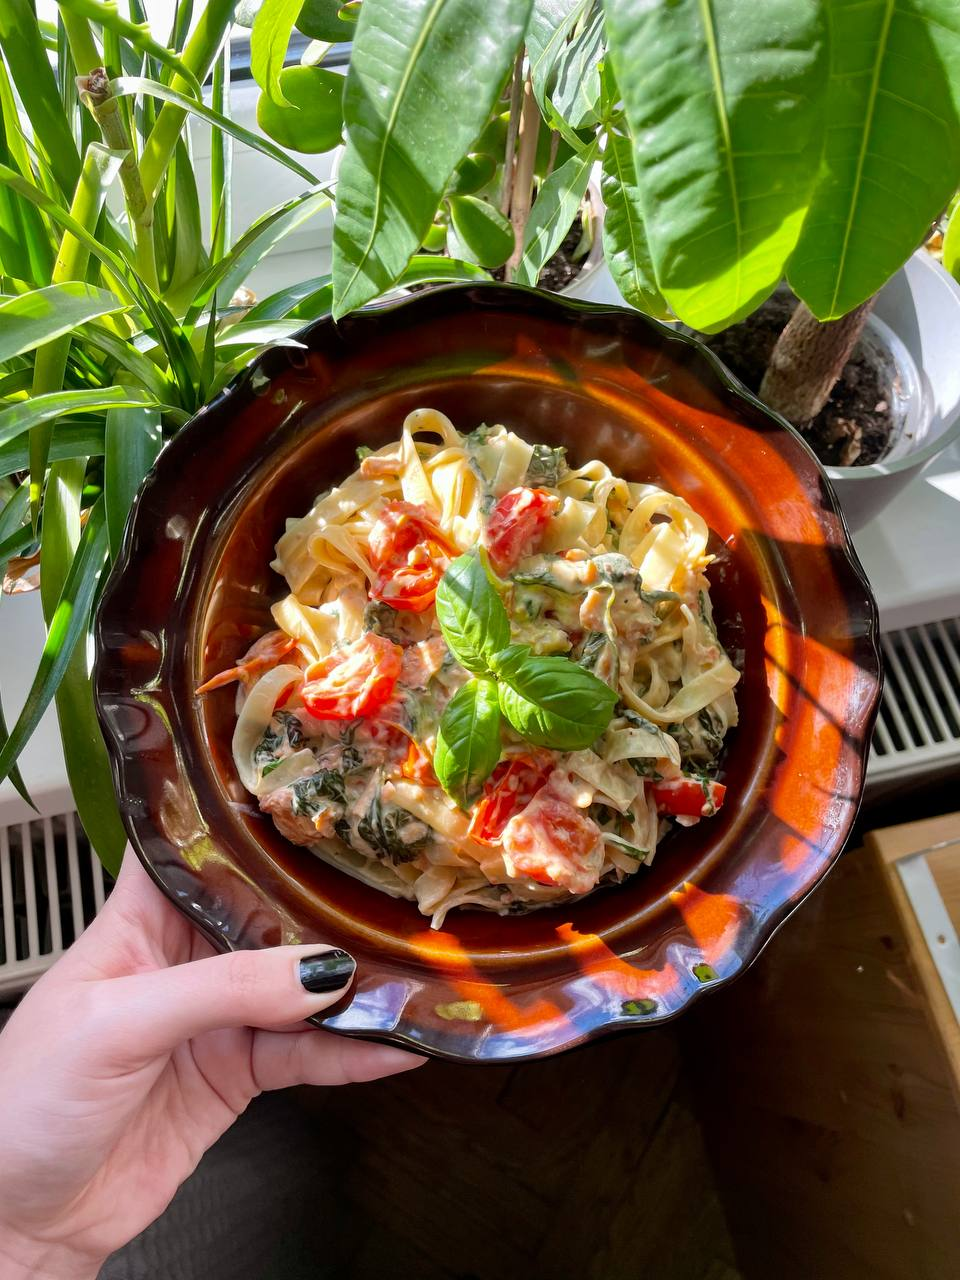
\includegraphics[width=0.35\textwidth]{images/makaron.jpg}}
\end{figure}
\end{multicols}

\vspace{0.5cm} 

\section*{Instruktaż:} \begin{enumerate} 
\item Pomidorki przekrojone w pól podsmażać na dobrze rozgrzanej patelni wraz ze szczyptą soli przez ok. 3 minuty, lub do momentu, aż się zarumienią. Dosypać szpinak i smażyć aż wytraci całą wodę.
\item Szpinak i pomidorki odsunąć na bok patelni, zmniejszyć moc palnika i na patelni podsmażyć wędzonego łososia poszarpanego na niewielkie kawałki przez ok. 3 minuty. Wszystko dokładnie wymieszać i na boku patelni delikatnie podsmażyć przeciśnięty przez praskę czosnek przez ok. 30 sekund. Całość zalać śmietanką, wymieszać i zagotować. Po zagotowaniu zmniejszyć na minimalny ogień i delikatnie dusić pod przykrywką przez ok. 10 minut, od czasu do czasu mieszając. 
\item W międzyczasie ugotować makaron zgodnie z instrukcją na opakowaniu i odcedzić. Ugotowany makaron przełożyć na patelnię z sosem, dokładnie wymieszać i doprawić odrobiną soli i pieprzu (uwaga na sól - wędzony łosoś jest zazwyczaj dość słony).
\end{enumerate}

\vspace{0.5cm}

\small \section*{Propozycja podania:} Ze startym serem, z listkami świeżej bazylii

\vspace{0.3cm}

\section*{Dodatkowe uwagi:} Szpinak i pomidorki można zastąpić innymi warzywami, również mrożonymi, np. brokułem, groszkiem, papryką, itp.

\chapter{Tofu na kuskusie z sezonową sałatką*}

\vspace{0.1cm}
\small
\begin{minipage}{0.45\textwidth}
    \noindent \textbf{Czas:} 30 minut \\
    \textbf{Poziom trudności:} umiarkowany
\end{minipage}
\begin{minipage}{0.45\textwidth}
    \noindent \textbf{Ilość sprzątania:} średnia\\
    \textbf{Wymagany mysi sprzęt:} -
\end{minipage}
\normalsize
\vspace{0.5cm}

\begin{multicols}{2}

\section*{Składniki:}
\begin{itemize}
    \item 1 porcja kaszy kuskus
    \item 0.75 kostki tofu (naturalnego, wędzonego, lub w gotowej marynacie)
    \item mix sałat  
    \item garść pomidorków koktajlowych lub 1 duży, dojrzały pomidor
    \item 1 ogórek gruntowy 
    \item 0.5 czerwonej cebuli
    \item zielona cebulka wedle uznania 
    \item 1 duży ząbek czosnku przeciśnięty przez praskę 
    \item 1 łyżka miodu
    \item przyprawy
    \item olej do smażenia
    \item odrobina oliwy i soku z cytryny
    \item 0.5 kostki bulionu warzywnego lub drobiowego
    \item sól i pieprz do smaku

\end{itemize}

\columnbreak

\begin{figure}[H]
    \centering
    \fbox{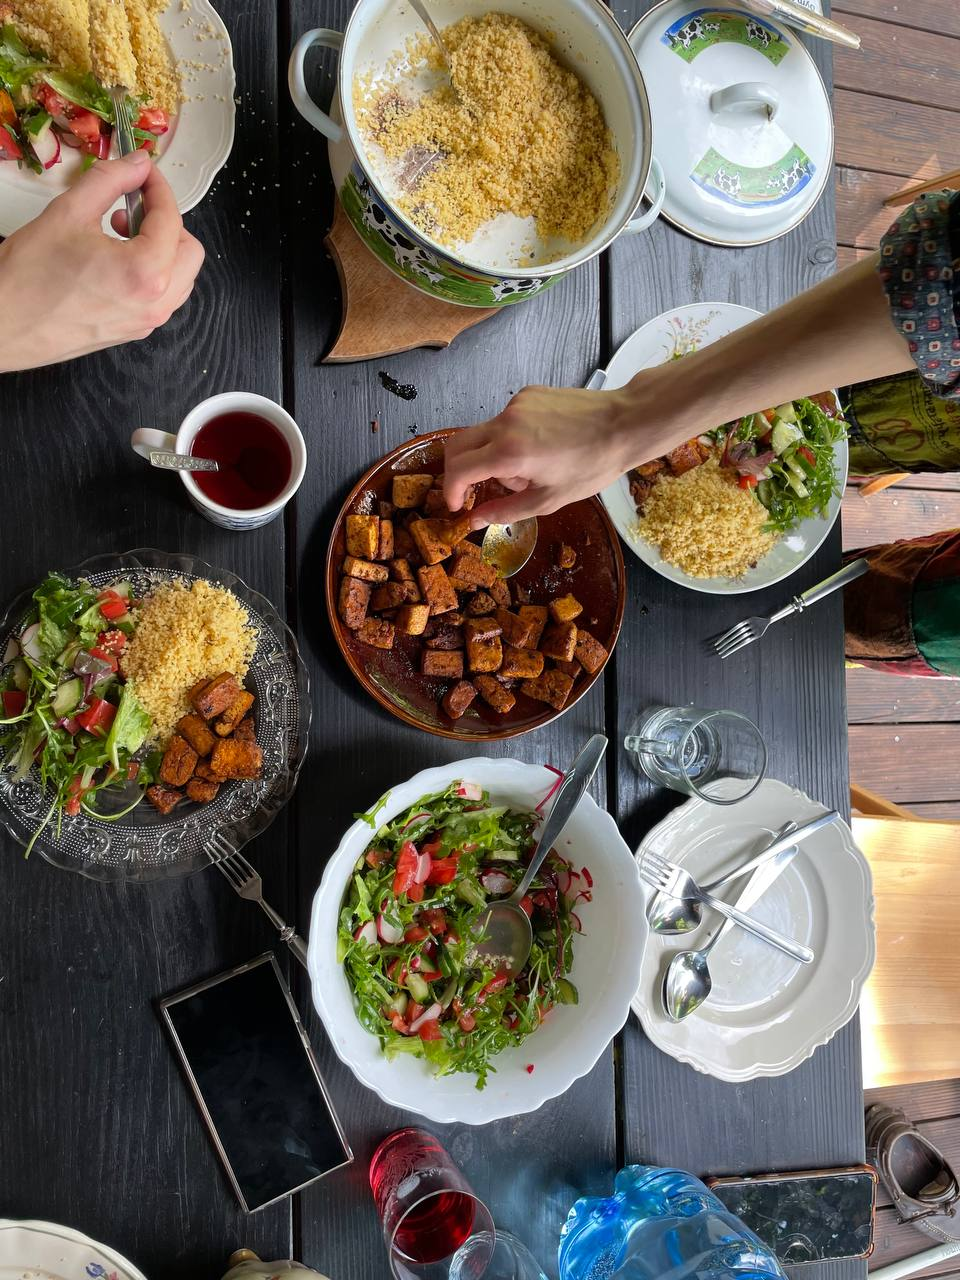
\includegraphics[width=0.45\textwidth]{images/tofu.jpg}}
\end{figure}
\end{multicols}

\vspace{0.5cm} 

\section*{Instruktaż:}
\begin{enumerate}
    \item Sałatkę i tofu przygotować osobno zgodnie z przepisem znajdującym się na ostatniej pozycji w spisie treści.
    \item W kubku odmierzyć odpowiednią porcję kaszy kuskus na 1 osobę i podsmażać wraz z połową łyżeczki pieprzu na niewielkiej ilości oliwy i małym ogniu do momentu zarumienienia się kaszy, lub przez ok. 3 minuty. Następnie zdjąć z ognia i zalać taką samą objętościowo ilością wody, uprzednio rozpuszczając w niej bulion i szczyptę soli. Całość przykryć i pozostawić na ok. 5 minut. 
    \item W razie potrzeby kaszę dosolić do smaku i podawać z tofu oraz sałatką
\end{enumerate}

\vspace{0.5cm} 

\small
\section*{Propozycja podania:}
Z posiekaną zieloną cebulką, z natką pietruszki, z domowym sosem czosnkowym

\vspace{0.3cm}

\section*{Dodatkowe uwagi:}
Nie mam uwag


\chapter{Domowa zupka typu instant*}

\vspace{0.1cm}
\small
\begin{minipage}{0.45\textwidth}
    \noindent \textbf{Czas:} 10 minut \\
    \textbf{Poziom trudności:} łatwy
\end{minipage}
\begin{minipage}{0.45\textwidth}
    \noindent \textbf{Ilość sprzątania:} minimalna\\
    \textbf{Wymagany mysi sprzęt:} -
\end{minipage}
\normalsize
\vspace{0.5cm}

\begin{multicols}{2}

\section*{Składniki:} \begin{itemize} 
\item cienki makaron ryżowy (lub inny pszenny typu instant) 
\item 2 łyżki sosu sojowego 
\item 1 łyżeczka pasty miso (opcjonalnie, aczkolwiek zalecane) 
\item 1/4 kostki bulionu warzywnego, drobiowego lub wołowego
\item 1/2 łyżeczki oleju sezamowego 
\item wybrane źródło białka (np. kostki tofu lub kawałki tzw. "kurczaka z rożna")
\item różne warzywa wedle uznania, świeże lub mrożone (np. floretki brokułu, cienkie paski marchewki, zielona cebulka, groszek zielony, itp.) 
\end{itemize}

\columnbreak

\begin{figure}[H]
    \centering
    \fbox{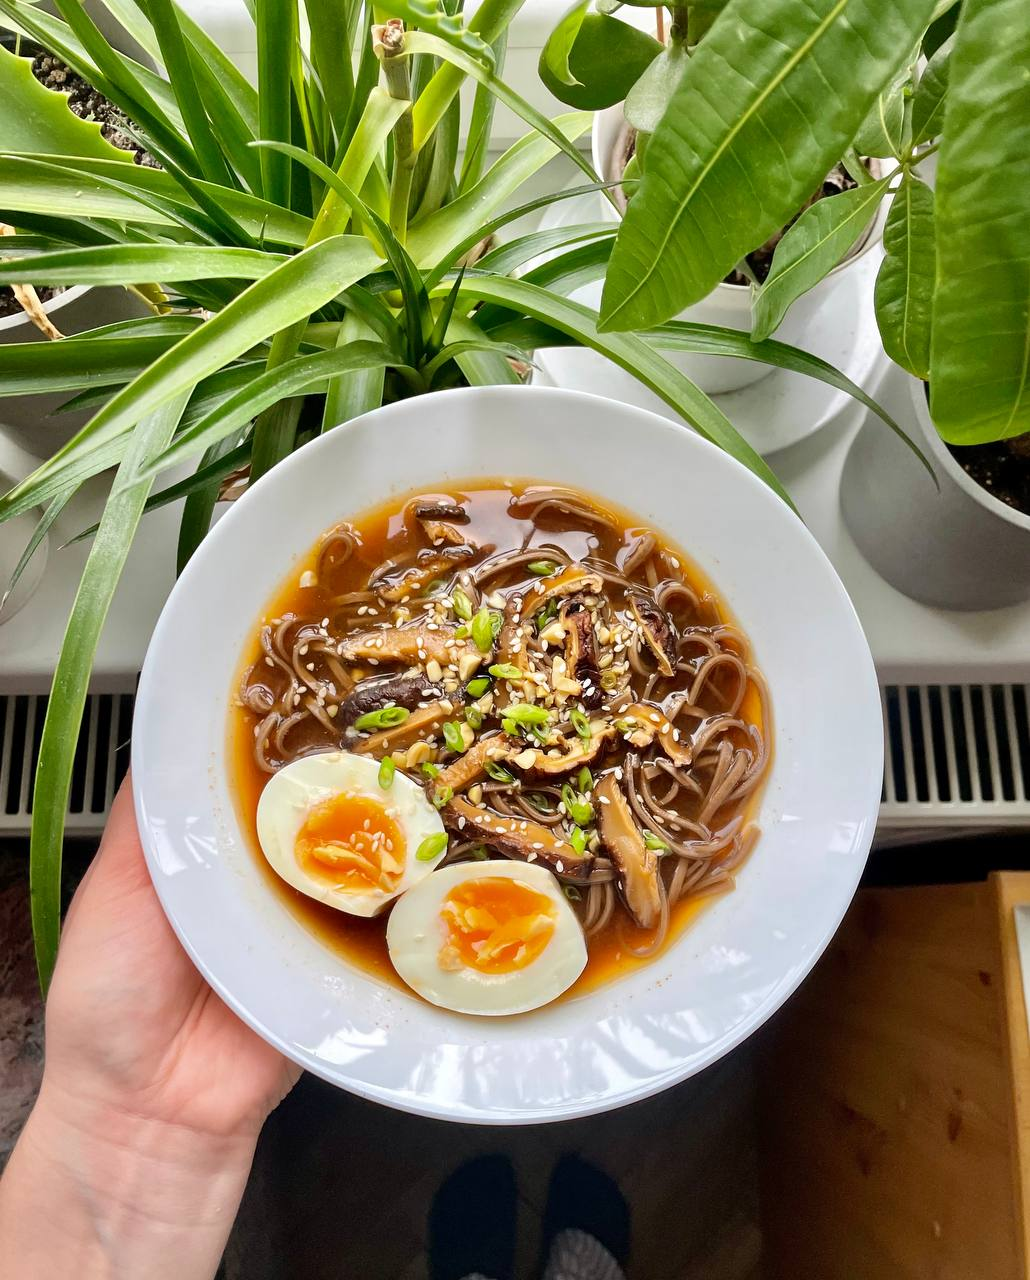
\includegraphics[width=0.35\textwidth]{images/zupka.jpg}}
\end{figure}
\end{multicols}

\vspace{0.5cm} 

\section*{Instruktaż:} \begin{enumerate} 
\item Na dnie średniej wielkości miski wymieszać ze sobą dokładnie sos sojowy, olej sezamowy, pastę i bulion. 
\item Warzywa pokroić na kawałki takiej wielkości, aby mogły ugotować się w kilka minut, tzn. marchewkę w drobną kostkę lub cienkie paski, brokuła rozdrobnić na małe floretki, itp. 
\item Pokrojone warzywa, tofu/kurczaka oraz makaron przełożyć do miski z sosem i zalać odpowiednią ilością wrzątku. Trzymać całość pod przykryciem przez ok. 5 minut lub do otrzymania pożądanej konsystencji makaronu. W razie potrzeby przyprawić do smaku sosem sojowym. 
\end{enumerate}

\vspace{0.5cm}

\small \section*{Propozycja podania:} Z jajkiem ugotowanym na miękko, z ziarenkami sezamu, z zieloną cebulką, z grzybami shiitake

\vspace{0.3cm}

\section*{Dodatkowe uwagi:} Danie można bardzo łatwo dostosować do wzięcia w drogę — wszystkie składniki wystarczy uprzednio włożyć do zamykanego pudełka na żywność wielokrotnego użytku lub szklanego słoika i zalać wrzątkiem w odpowiedniej chwili

\chapter{Błyskawiczny makaron w sosie orzechowym*}

\vspace{0.1cm}
\small
\begin{minipage}{0.45\textwidth}
    \noindent \textbf{Czas:} 10 minut \\
    \textbf{Poziom trudności:} łatwy
\end{minipage}
\begin{minipage}{0.45\textwidth}
    \noindent \textbf{Ilość sprzątania:} minimalna\\
    \textbf{Wymagany mysi sprzęt:} blender (opcjonalnie)
\end{minipage}
\normalsize
\vspace{0.5cm}

\begin{multicols}{2}

\section*{Składniki:} 
\begin{itemize} 
\item porcja makaronu ryżowego (można też użyć pszennego) 
\item 2 łyżki masła orzechowego 
\item 1 duży lub 2 małe ząbki czosnku, przeciśnięte przez praskę 
\item 1 łyżka sosu sojowego 
\item 1/2 - 1 łyżka ostrego sosu typu sriracha 
\item odrobina wyciśniętego soku z cytryny 
\item 1 łyżka miodu lub cukru 
\item 5 łyżek wrzątku lub wody spod makaronu
\item 1 łyżeczka oleju sezamowego 
\end{itemize}

\columnbreak

\begin{figure}[H] \centering 
 \fbox{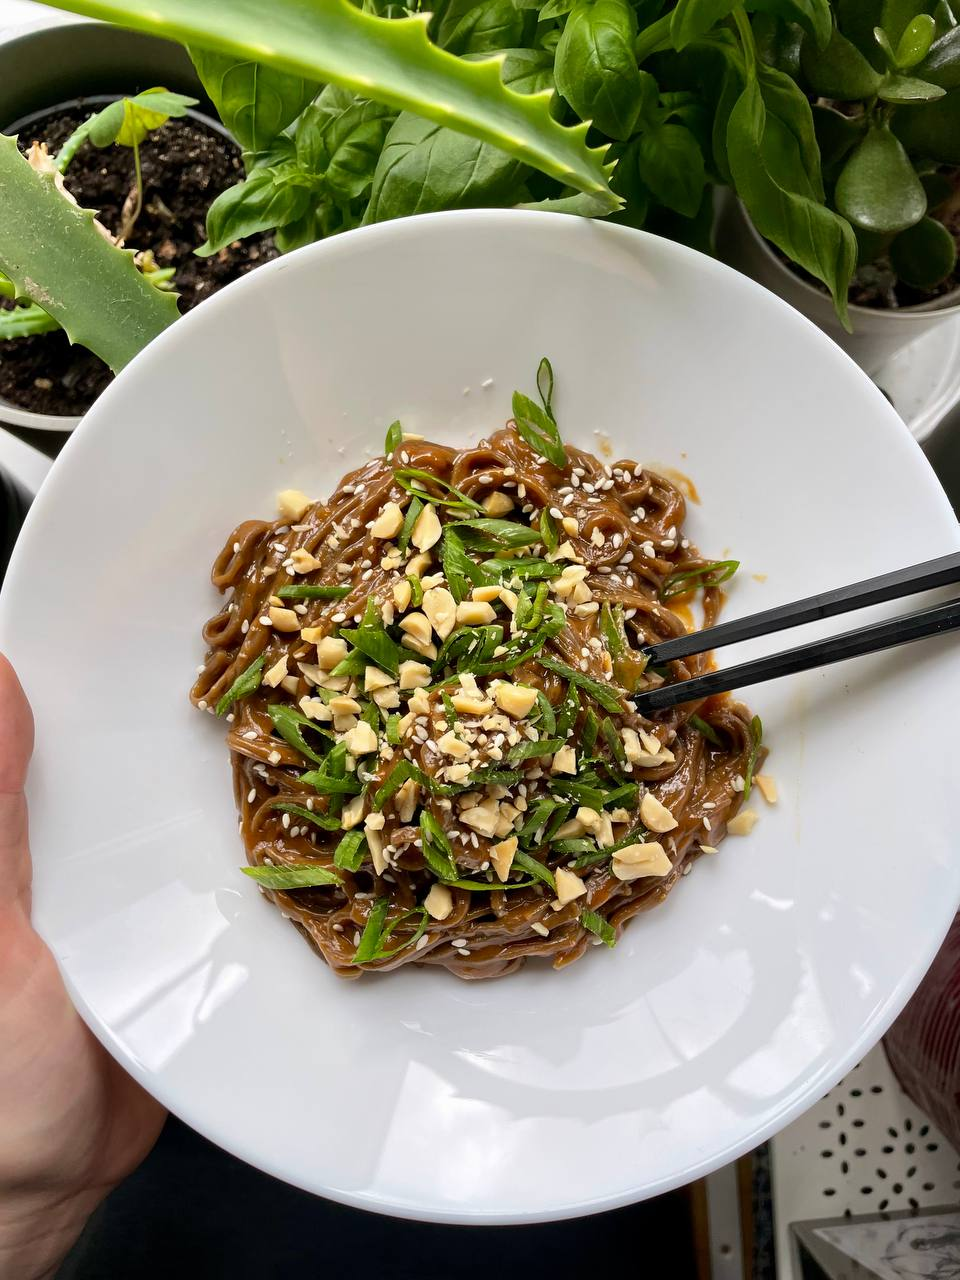
\includegraphics[width=0.35\textwidth]{images/makaronorzechowy.jpg}}
\end{figure}

\end{multicols}

\vspace{0.5cm}

\section*{Instruktaż:} 
\begin{enumerate} 
\item Zagotować osoloną wodę na makaron i gotować według instrukcji na opakowaniu.
\item W międzyczasie połączyć resztę składników w niewielkiej miseczce i dokładnie wymieszać lub zblendować na gładki sos. 
\item Makaron odcedzić i przełożyć z powrotem do garnka. Wymieszać z sosem i ewentualnie podgrzać. 
\end{enumerate}

\vspace{0.5cm}

\small \section*{Propozycja podania:} Z orzeszkami ziemnymi, z posiekaną zieloną cebulką, z nasionkami sezamu

\vspace{0.3cm}

\section*{Dodatkowe uwagi:} W celu zwiększenia ilości białka w daniu do makaronu można dodać usmażone na chrupko tofu bądź kawałki kurczaka

\chapter{Pieczona fasolka szparagowa*}

\vspace{0.1cm}
\small
\begin{minipage}{0.45\textwidth}
    \noindent \textbf{Czas:} 45 minut \\
    \textbf{Poziom trudności:} łatwy
\end{minipage}
\begin{minipage}{0.45\textwidth}
    \noindent \textbf{Ilość sprzątania:} średnia\\
    \textbf{Wymagany mysi sprzęt:} piekarnik
\end{minipage}
\normalsize
\vspace{0.5cm}

\begin{multicols}{2}

\section*{Składniki:}
\begin{itemize}
    \item szczodra garść fasolki szparagowej
    \item 1 łyżeczka skórki z limonki
    \item 3 łyżki orzeszków ziemnych
    \item 4 łyżki oliwy 
    \item 0.25 łyżeczki płatków chilli lub pieprzu cayenne
    \item mała garstka świeżej kolendry (można zastąpić listkami bazylii, mięty, lub pietruszki)
    \item sól do smaku
\end{itemize}

\columnbreak

\begin{figure}[H]
    \centering
    \fbox{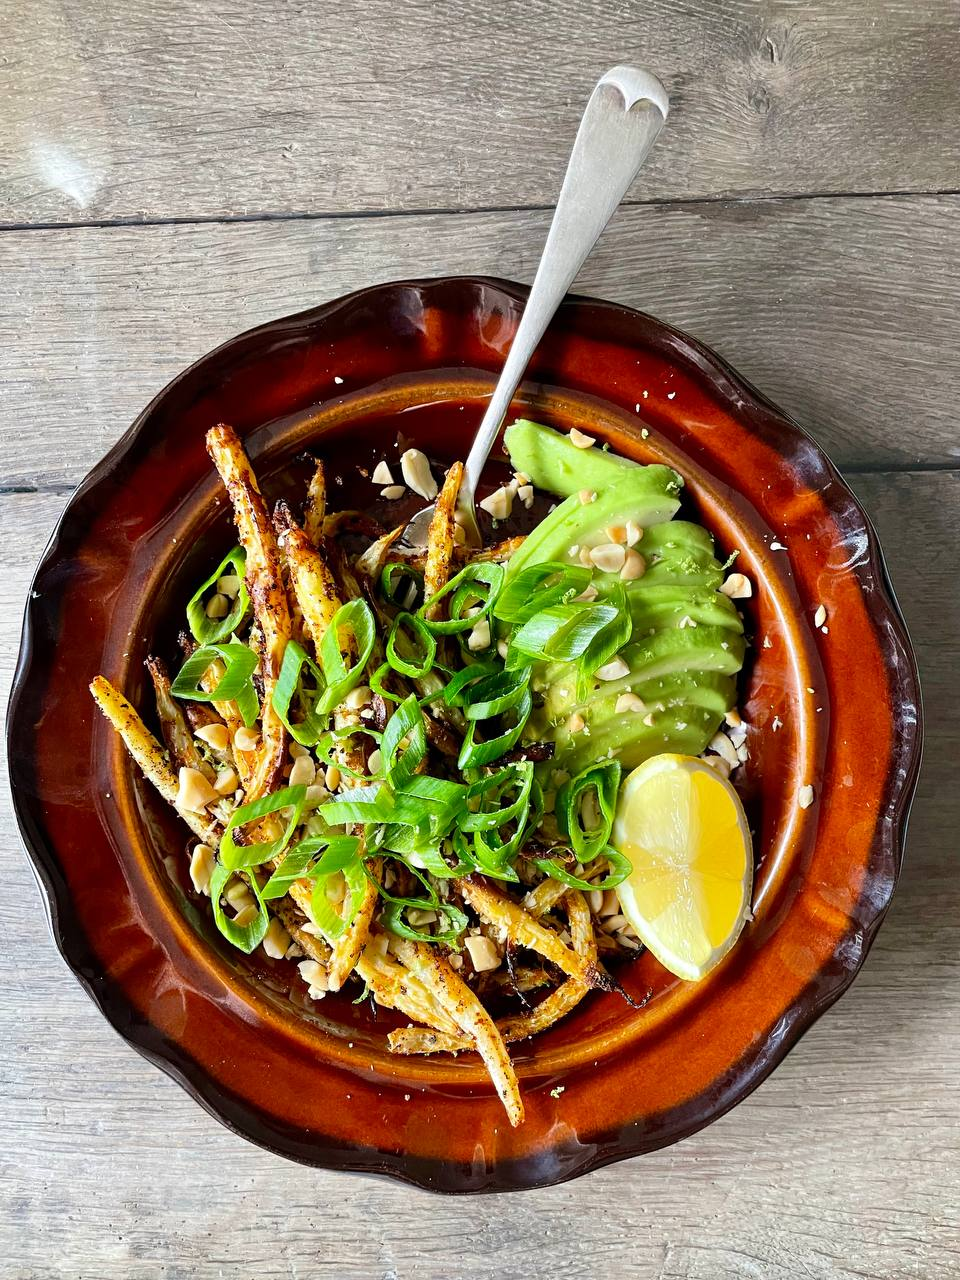
\includegraphics[width=0.35\textwidth]{images/fasolkaszparagowa.jpg}}
\end{figure}
\end{multicols}

\vspace{0.5cm} 

\section*{Instruktaż:}
\begin{enumerate}
    \item Piekarnik rozgrzać do 220 stopni Celsjusza i blaszkę wyłożyć papierem do pieczenia
    \item Odciąć zdrewniałe końcówki z fasolki szparagowej i przełożyć na blaszkę wraz z skórką z limonki, chili oraz hojną szczyptą soli. Skropić oliwą i dokładnie obtoczyć fasolkę w marynacie – najlepiej rękami.
    \item Piec przez 30 – 40 minut, aż fasolka będzie miękka i częściowo poczernieje na brzegach.
    \item Po upieczeniu dodać orzeszki ziemne oraz kolendrę i dokładnie wymieszać. 
\end{enumerate}

\vspace{0.5cm} 

\small
\section*{Propozycja podania:}
Ze świeżym sokiem z limonki, z bułką tartą podsmażoną na maśle, z awokado, jako dodatek do obiadu

\vspace{0.3cm}

\section*{Dodatkowe uwagi:}
Fasolkę najlepiej podawać zaraz po upieczeniu, aby nie traciła na chrupkości

\chapter{Ciecierzyca w sosie curry*}

\vspace{0.1cm}
\small
\begin{minipage}{0.45\textwidth}
    \noindent \textbf{Czas:} 45 minut \\
    \textbf{Poziom trudności:} łatwy 
\end{minipage}
\begin{minipage}{0.45\textwidth}
    \noindent \textbf{Ilość sprzątania:} minimalna\\
    \textbf{Wymagany mysi sprzęt:} -
\end{minipage}
\normalsize
\vspace{0.5cm}

\begin{multicols}{2}

\section*{Składniki:} \begin{itemize} 
\item 1 duża cebula 
\item 2 łyżeczki nasion gorczycy (albo graniastej musztardy francuskiej) 
\item 1 puszka mleka kokosowego (opcjonalnie dodatkowo: małe opakowanie śmietany 18\%) 
\item 1 puszka krojonych pomidorów 
\item 3 puszki ciecierzycy 
\item 2 łyżki sosu sojowego 
\item 1-2 łyżeczki cukru trzcinowego (lub zwykłego) 
\item przyprawy 
\item olej do smażenia 
\item sól i pieprz do smaku
\end{itemize}

\columnbreak

\begin{figure}[H] \centering \fbox{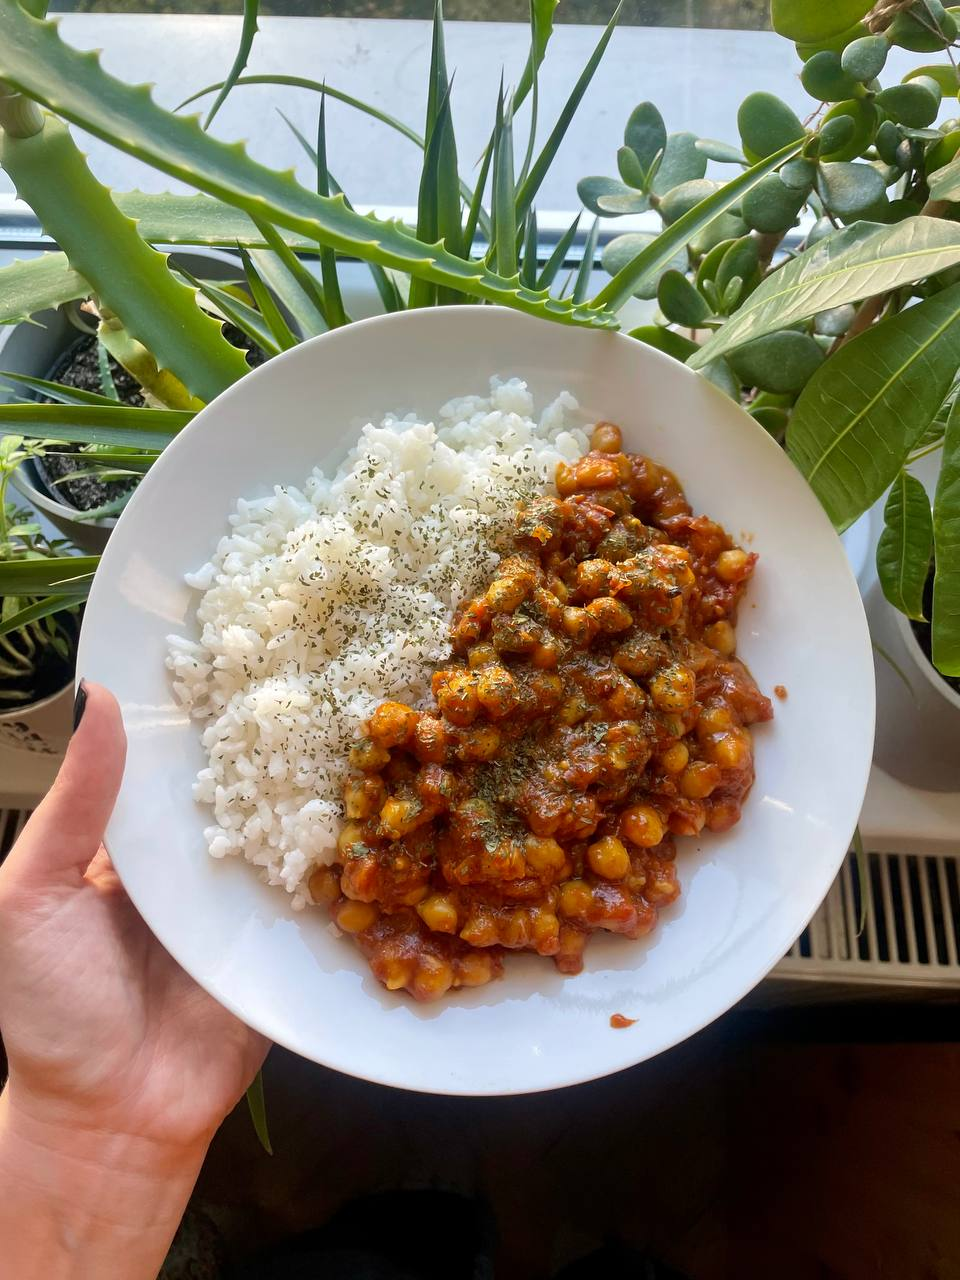
\includegraphics[width=0.35\textwidth]{images/curry.jpg}} \end{figure}

\end{multicols}

\vspace{0.5cm}

\section*{Instruktaż:} \begin{enumerate} \item Cebulę posiekać na drobne kawałki i podsmażać do zeszklenia na oleju wraz z ziarnami gorczycy/musztardą i hojną szczyptą soli. \item Przez 30 sekund podsmażać przyprawy: po 2 łyżeczki kminu rzymskiego i curry, 1 łyżeczka kurkumy, chilli zgodnie z pożądanym poziomem ostrości (0.5-1 łyżeczka), hojna szczypta cynamonu. \item Wstrząsnąć puszkę z mlekiem kokosowym i wlać ją do garnka, dodać pomidory oraz sos sojowy i cukier. Dokładnie wymieszać i gotować aż zgęstnieje na średnim ogniu przez ok. 30 minut od momentu, gdy zacznie wrzeć, mieszając od czasu do czasu. \item Po upływie 30 minut dosolić do smaku, odsączyć ciecierzycę, wsypać do garnka i gotować na średnim ogniu ok. 15 minut, aż do uzyskania pożądanej konsystencji. \end{enumerate}

\vspace{0.5cm}

\small \section*{Propozycja podania:} Ze świeżą kolendrą, z ryżem, z chlebkami indyjskimi naan z patelni

\vspace{0.3cm}

\section*{Dodatkowe uwagi:} Smakuje wybornie zarówno na zimno, jak i ciepło. Idealne do wzięcia w drogę lub do szkoły :)



\chapter{Sałatka z tofu*/kurczakiem}

\vspace{0.1cm}
\small
\begin{minipage}{0.45\textwidth}
    \noindent \textbf{Czas:} 30 minut \\
    \textbf{Poziom trudności:} umiarkowany
\end{minipage}
\begin{minipage}{0.45\textwidth}
    \noindent \textbf{Ilość sprzątania:} średnia\\
    \textbf{Wymagany mysi sprzęt:} -
\end{minipage}
\normalsize
\vspace{0.5cm}

\begin{multicols}{2}

\section*{Składniki:}
\begin{itemize}
    \item 1 pierś z kurczaka (lub odpowiadająca ilość tofu)
    \item mix sałat  
    \item garść pomidorków koktajlowych lub 1 duży, dojrzały pomidor
    \item 1 ogórek gruntowy 
    \item 0.5 czerwonej cebuli
    \item zielona cebulka wedle uznania 
    \item garść kiełków brokułu (opcjonalnie) 
    \item 1 duży ząbek czosnku przeciśnięty przez praskę 
    \item 1 łyżka miodu
    \item przyprawy
    \item olej do smażenia
    \item odrobina oliwy i soku z cytryny
    \item sól i pieprz do smaku
\end{itemize}

\columnbreak

\begin{figure}[H]
    \centering
    \fbox{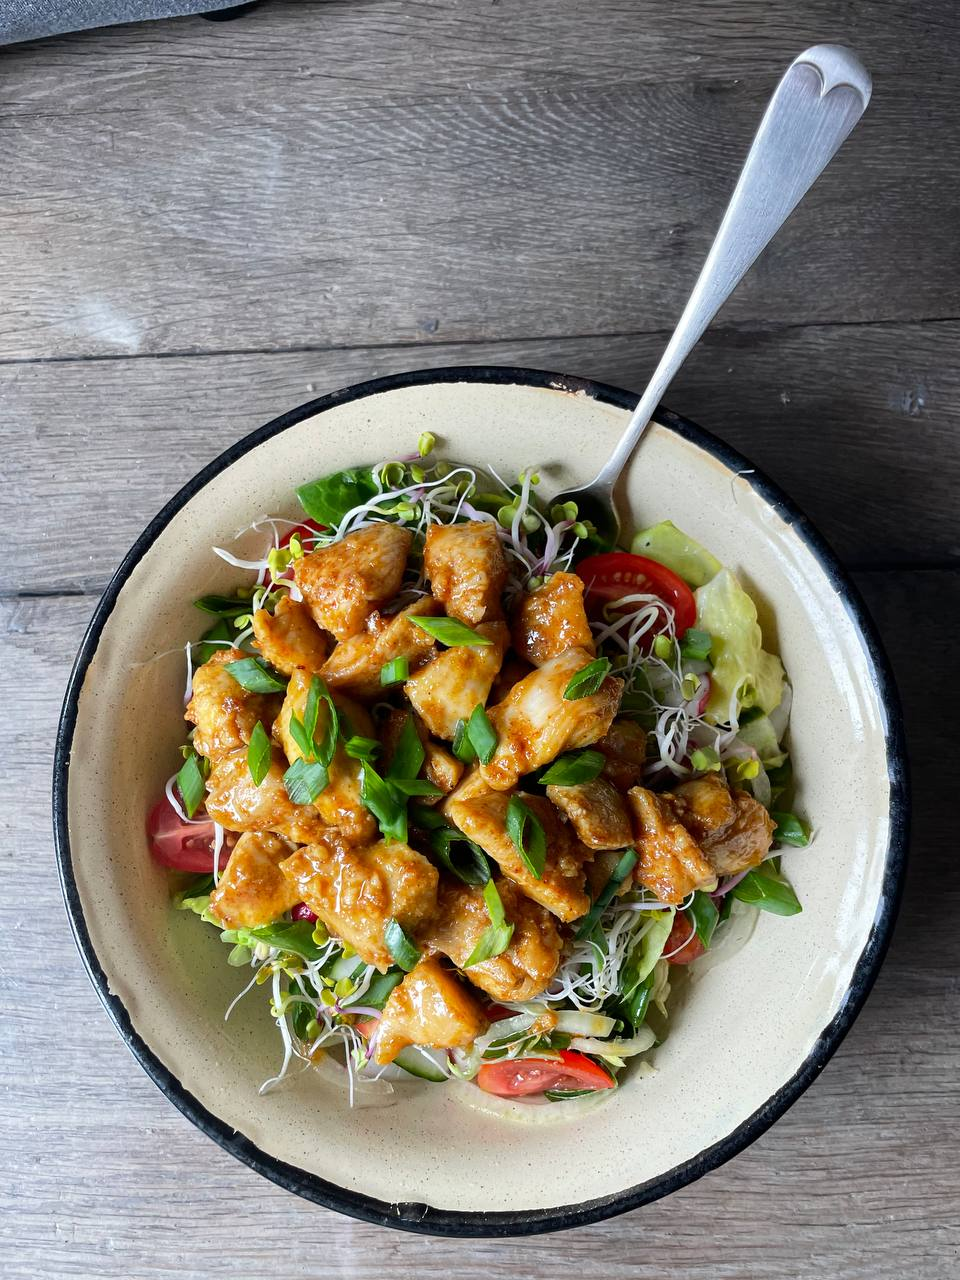
\includegraphics[width=0.4\textwidth]{images/salatka.jpg}} 
\end{figure}
\end{multicols}

\vspace{0.5cm} 

\section*{Instruktaż:}
\begin{enumerate}
    \item Kurczaka/tofu pokroić w średniej wielkości kostkę, przełożyć do niewielkiej miski i doprawić po 1/2 łyżeczki solą oraz pieprzem. dołożyć czosnek i następująco po 1 płaskiej łyżeczce: oliwy, papryki słodkiej, bazylii, oregano, majeranku i przyprawy do kurczaka. wymieszać dokładnie pozostawić do marynowania na ok. 10 minut. 
    \item W międzyczasie pokroić ogórka, pomidorki na połówki i cebulę w piórka. do dużej miski nałożyć garść sałaty i dosypać pokrojone wcześniej warzywa oraz kiełki. całość doprawić solą, pieprzem, oliwą i sokiem z cytryny. wszystko bardzo dokładnie wymieszać.
    \item Patelnię rozgrzać na średnim ogniu wraz z niewielką ilością oleju. kurczaka smażyć krótko, ok. 3 min na każdą stronę, aż do momentu uzyskania jednolitego koloru wewnątrz kawałków. tofu smażyć dłużej, ok. 15 minut, często mieszając, do momentu uzyskania chrupkiej warstwy zewnętrznej (można pomóc dodając 2 łyżeczki skrobii ziemniaczanej). 
    \item po upływie odpowiedniego czasu zgasić palnik, doprawić kurczaka/tofu łyżką miodu, całość dokładnie wymieszać i pozostawić do ostudzenia.
    \item Na sałatę nałożyć kurczaka/tofu i posypać posiekaną zieloną cebulką
\end{enumerate}

\vspace{0.5cm} 

\small
\section*{Propozycja podania:}
Ze świeżym pieczywem i masłem/oliwą, jako dodatek do obiadu

\vspace{0.3cm}

\section*{Dodatkowe uwagi:}
• do sałatki warto dodać sezonowe warzywa wedle własnego uznania, np. rzodkiewkę, paprykę, marchewkę, awokado, itp. 
 • aby ostry smak surowej czerwonej cebuli nie przytłaczał pozostałych składników, warto ją sparzyć - czyli pokrojoną już w piórka wrzucić do niewielkiej miseczki i zalać wrzątkiem na kilka minut. to spowoduje, że cebula w potrawach zachowa swój pyszny smak, a jednocześnie zaniknie jej nieprzyjemna ostrość

 \chapter{Inspiracje}

 \begin{figure}[H]
    \centering
    \begin{minipage}{0.4\textwidth}
        \centering
        \fbox{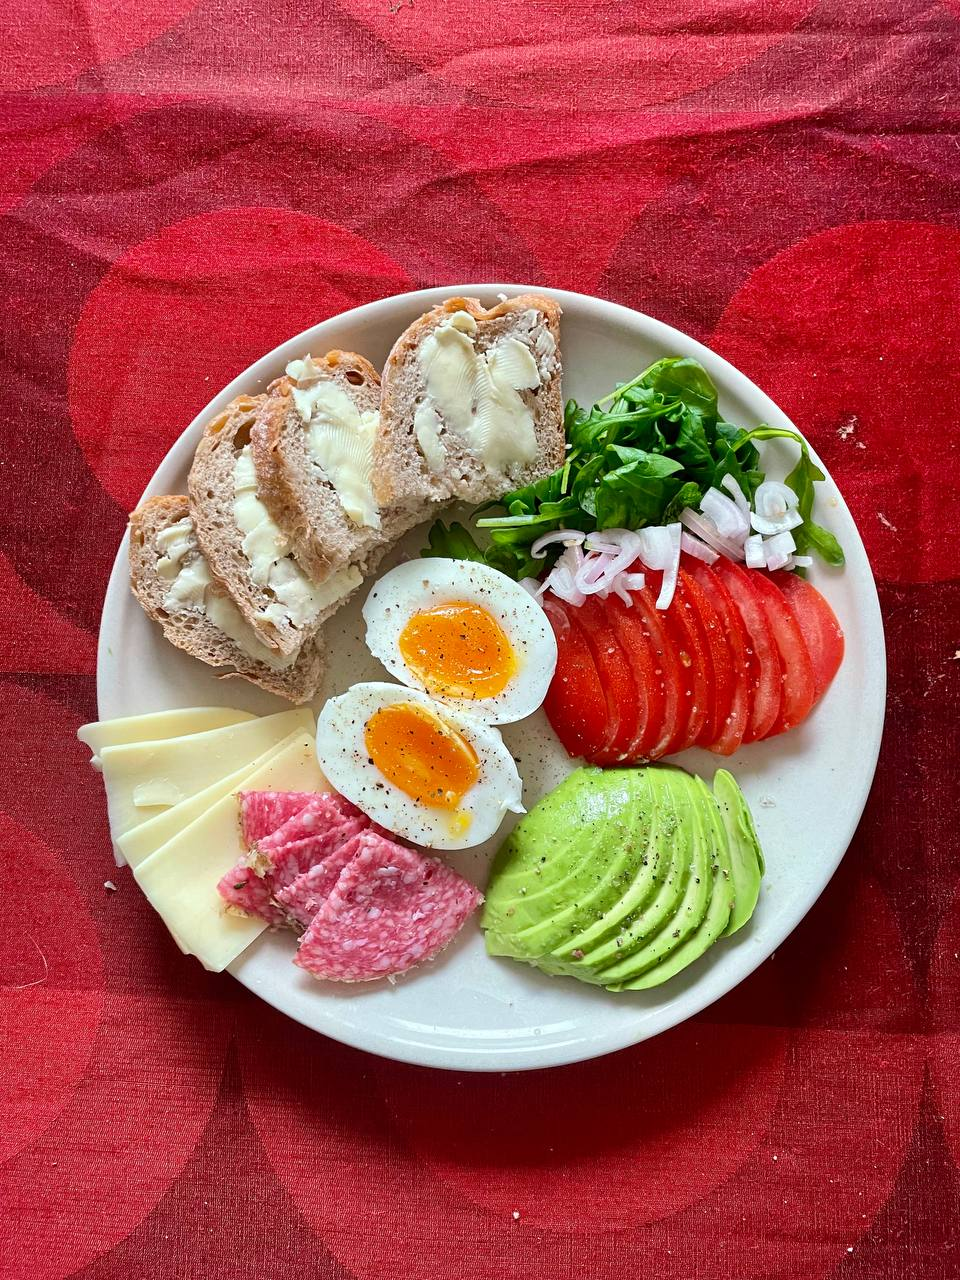
\includegraphics[width=\textwidth]{images/sample1.jpg}}
        \caption{Indywidualny szwedzki stół}
    \end{minipage}
    \hspace{0.05\textwidth}
    \begin{minipage}{0.4\textwidth}
        \centering
        \fbox{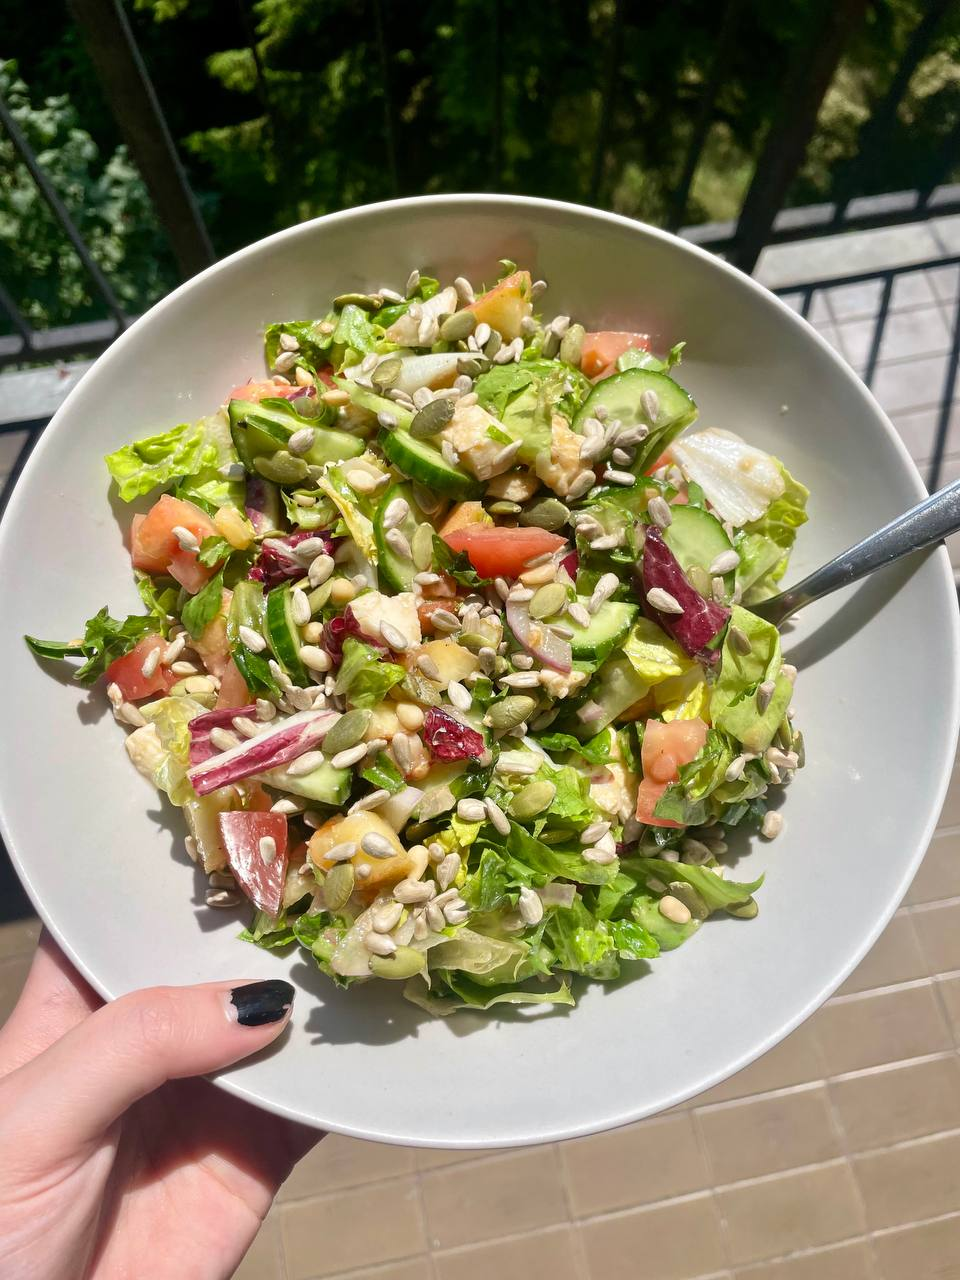
\includegraphics[width=\textwidth]{images/sample2.jpg}} 
        \caption{Sezonowa sałatka z brzoskwinią i orzeszkami}
    \end{minipage}
    
    \vspace{0.05\textwidth}
    
    \begin{minipage}{0.4\textwidth}
        \centering
        \fbox{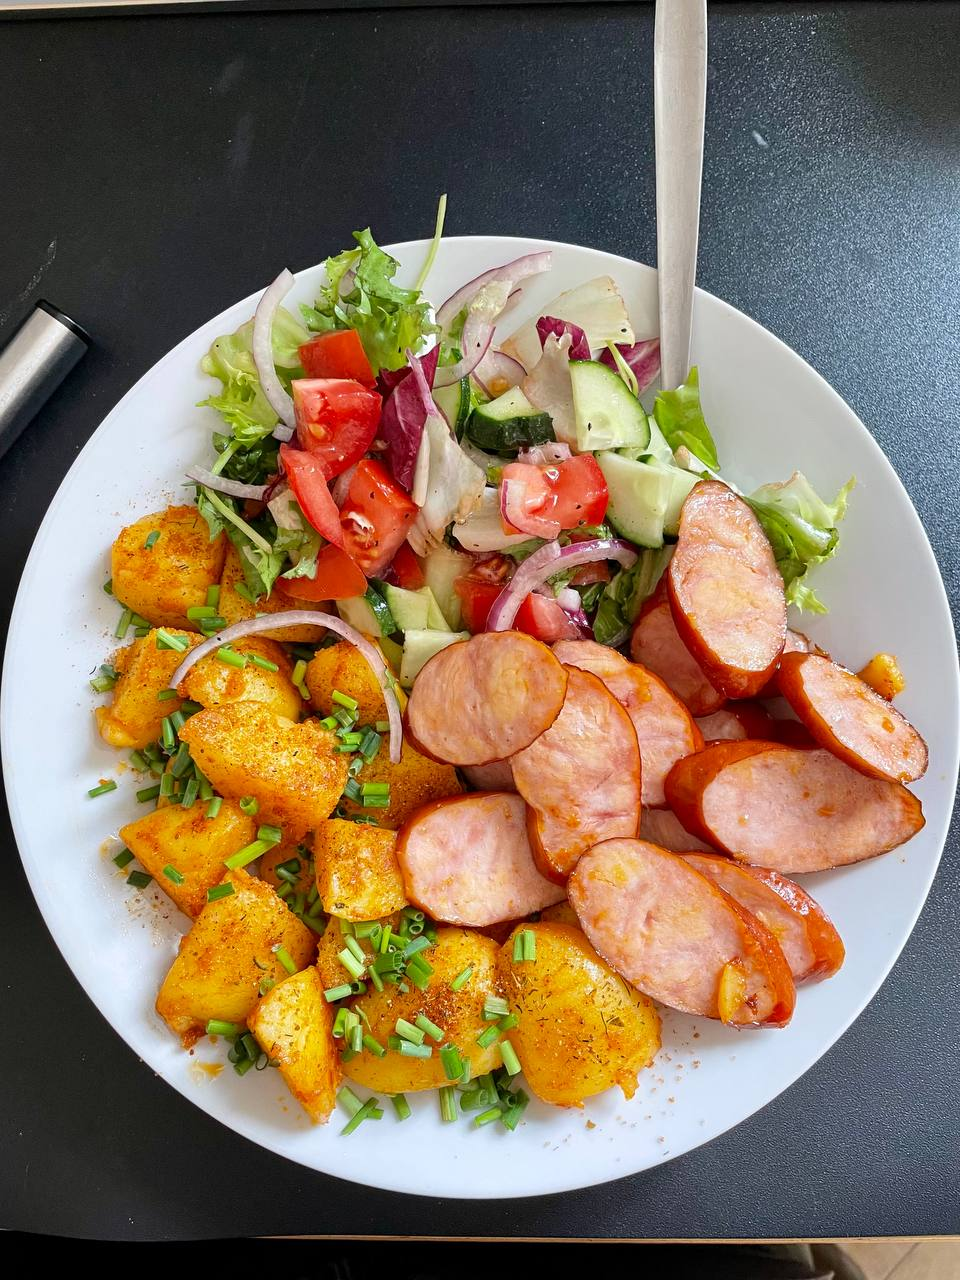
\includegraphics[width=\textwidth]{images/sample3.jpg}} 
        \caption{Smażona kiełbasa z ziemniaczkami i sałatką}
    \end{minipage}
    \hspace{0.05\textwidth} 
    \begin{minipage}{0.4\textwidth}
        \centering
        \fbox{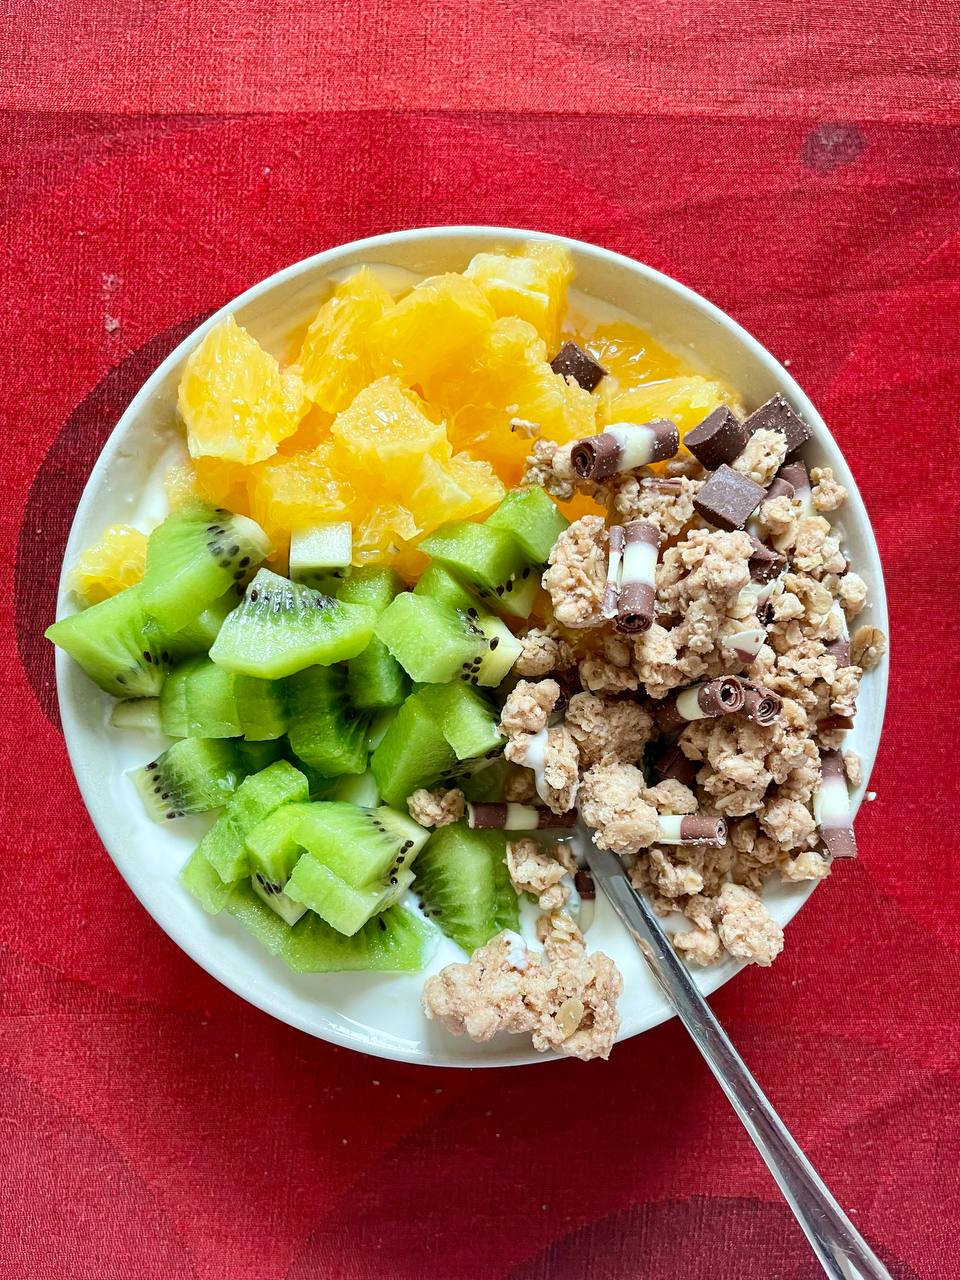
\includegraphics[width=\textwidth]{images/sample5.jpg}} 
        \caption{Jogurt z sezonowymi owocami zimowymi}
    \end{minipage}
    
\end{figure}

\newpage

\begin{figure}[H]
    \centering
    \begin{minipage}{0.4\textwidth}
        \centering
        \fbox{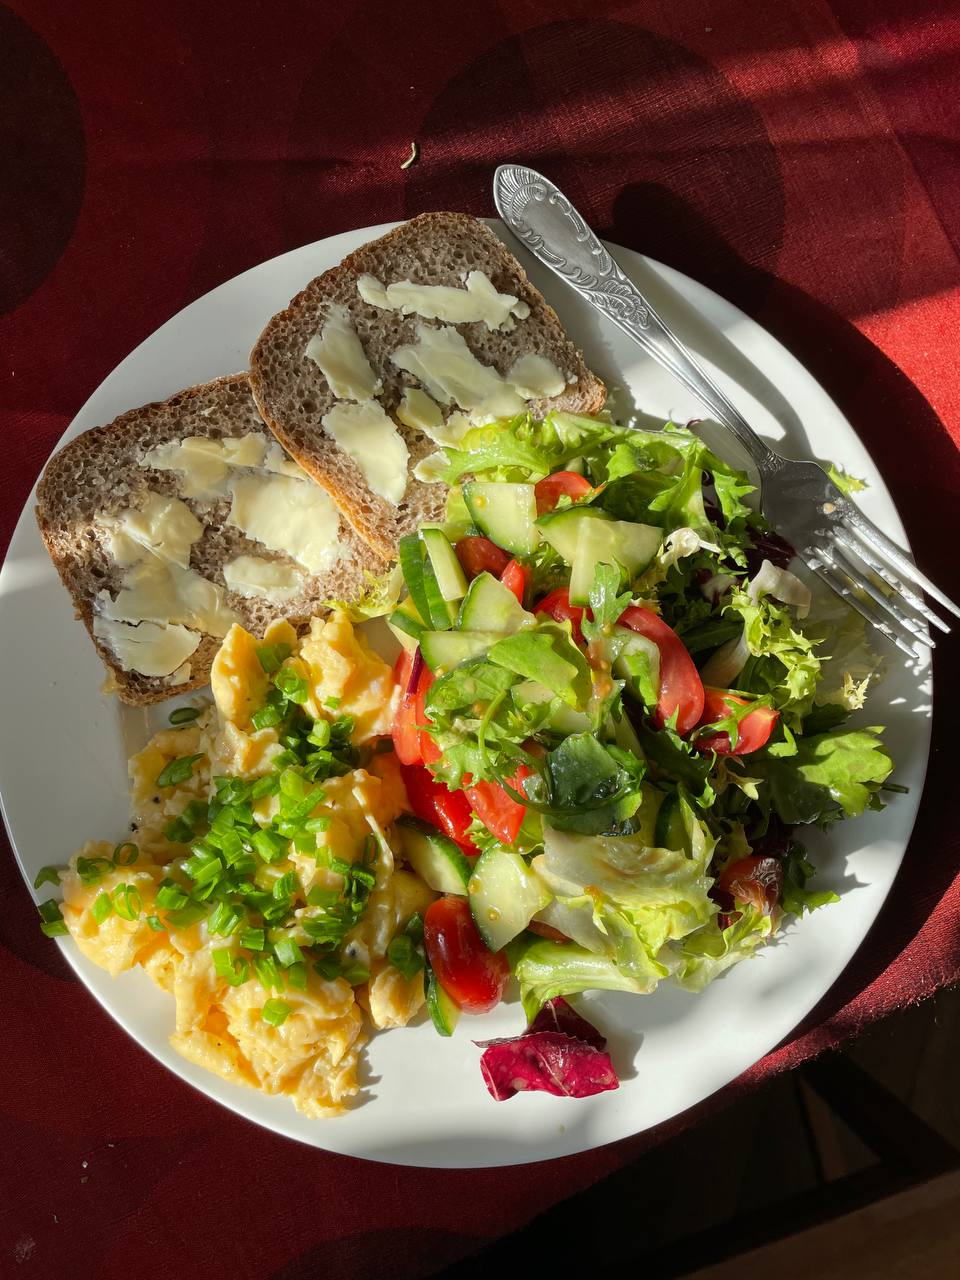
\includegraphics[width=\textwidth]{images/sample4.jpg}}
        \caption{Jajecznica na maśle z chlebem żytnim i warzywami}
    \end{minipage}
    \hspace{0.05\textwidth}
    \begin{minipage}{0.4\textwidth}
        \centering
        \fbox{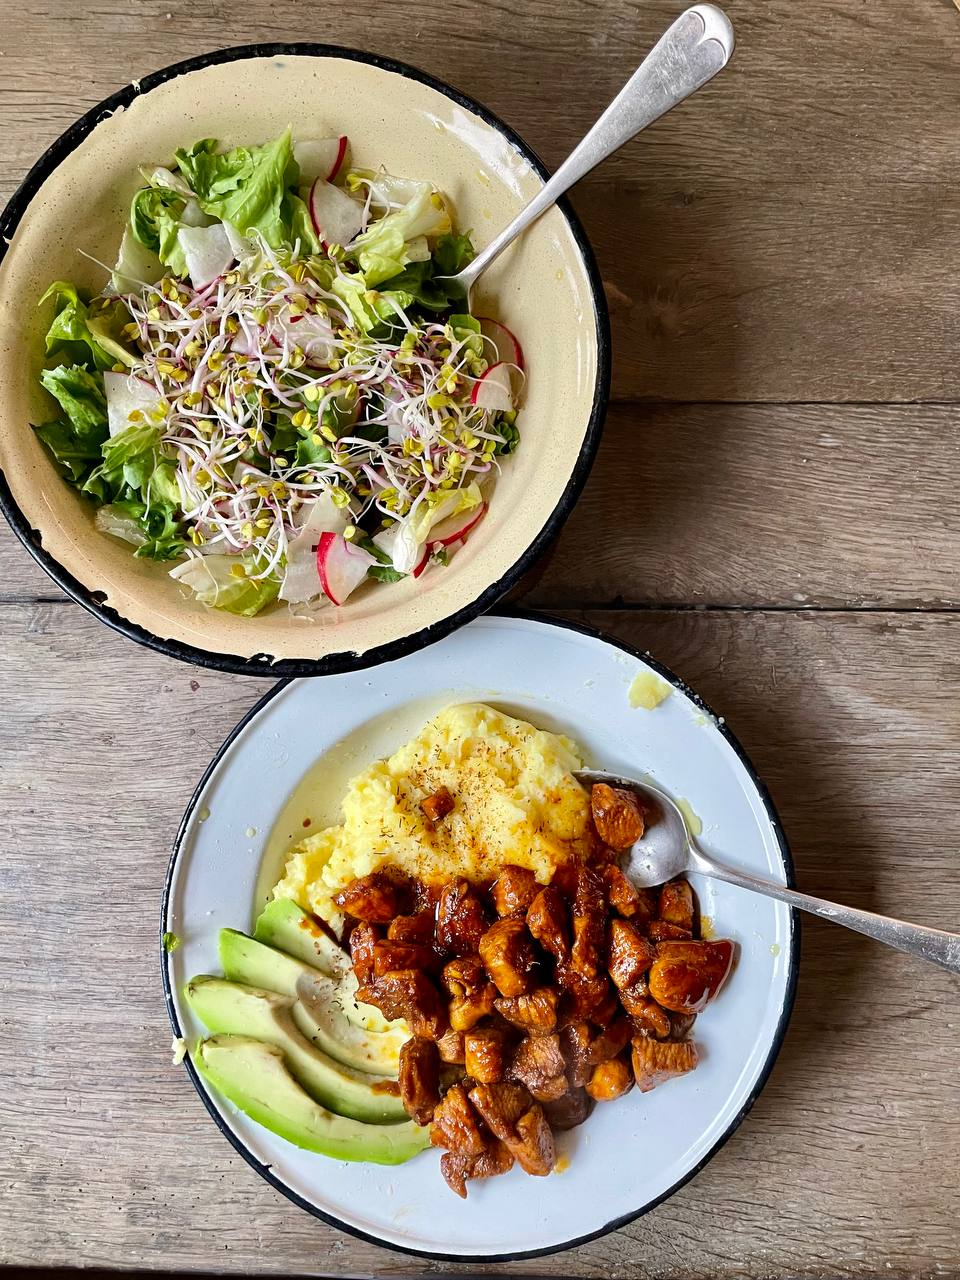
\includegraphics[width=\textwidth]{images/sample9.jpg}} 
        \caption{Kurczak w sosie słodko-ostrym z puree ziemniaczanym i sałatką}
    \end{minipage}
    
    \vspace{0.05\textwidth}
    
    \begin{minipage}{0.4\textwidth}
        \centering
        \fbox{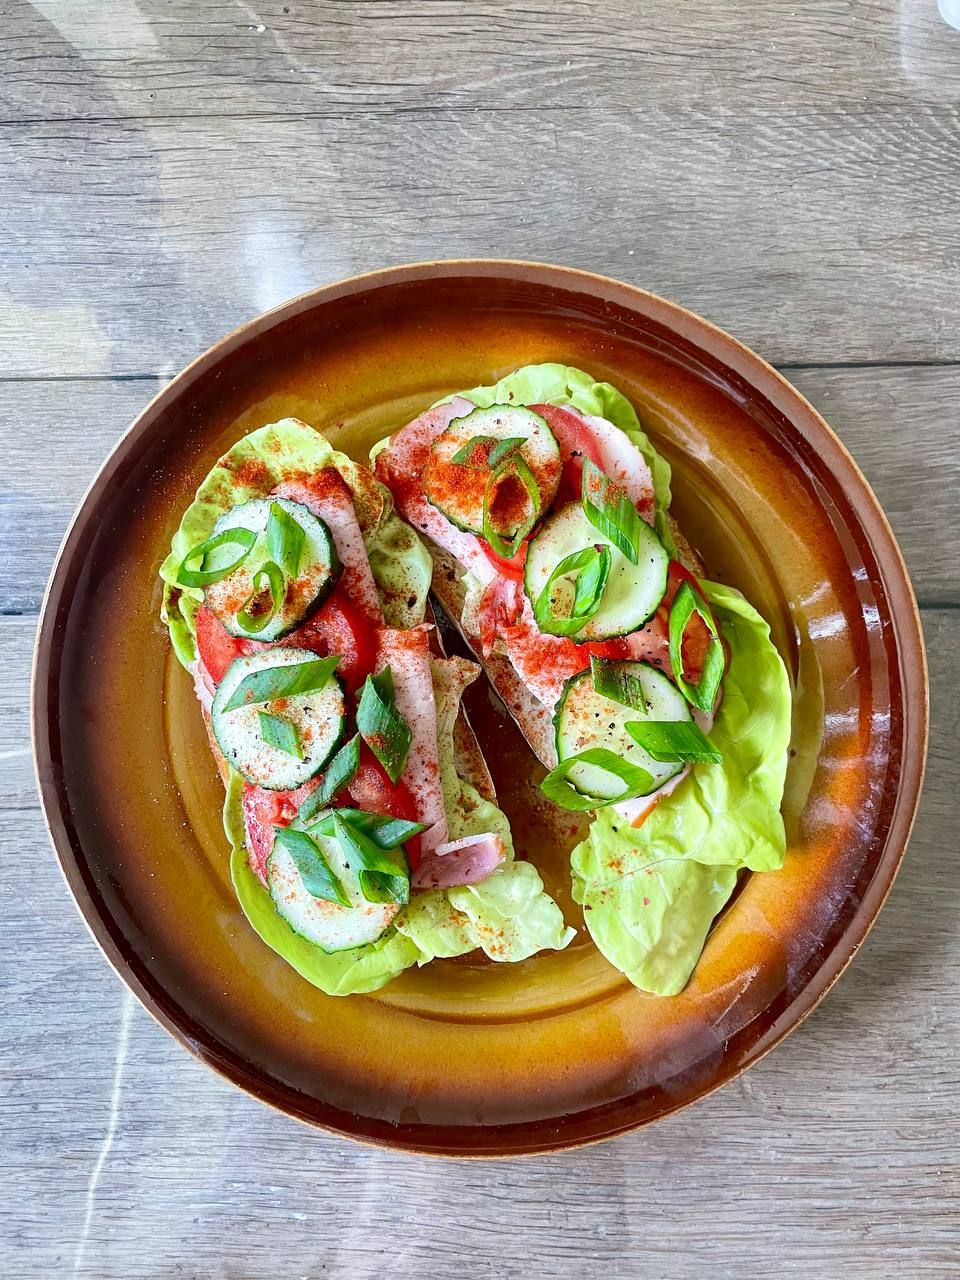
\includegraphics[width=\textwidth]{images/sample7.jpg}} 
        \caption{Wiosenne kanapki z wędliną i warzywami}
    \end{minipage}
    \hspace{0.05\textwidth} 
    \begin{minipage}{0.4\textwidth}
        \centering
        \fbox{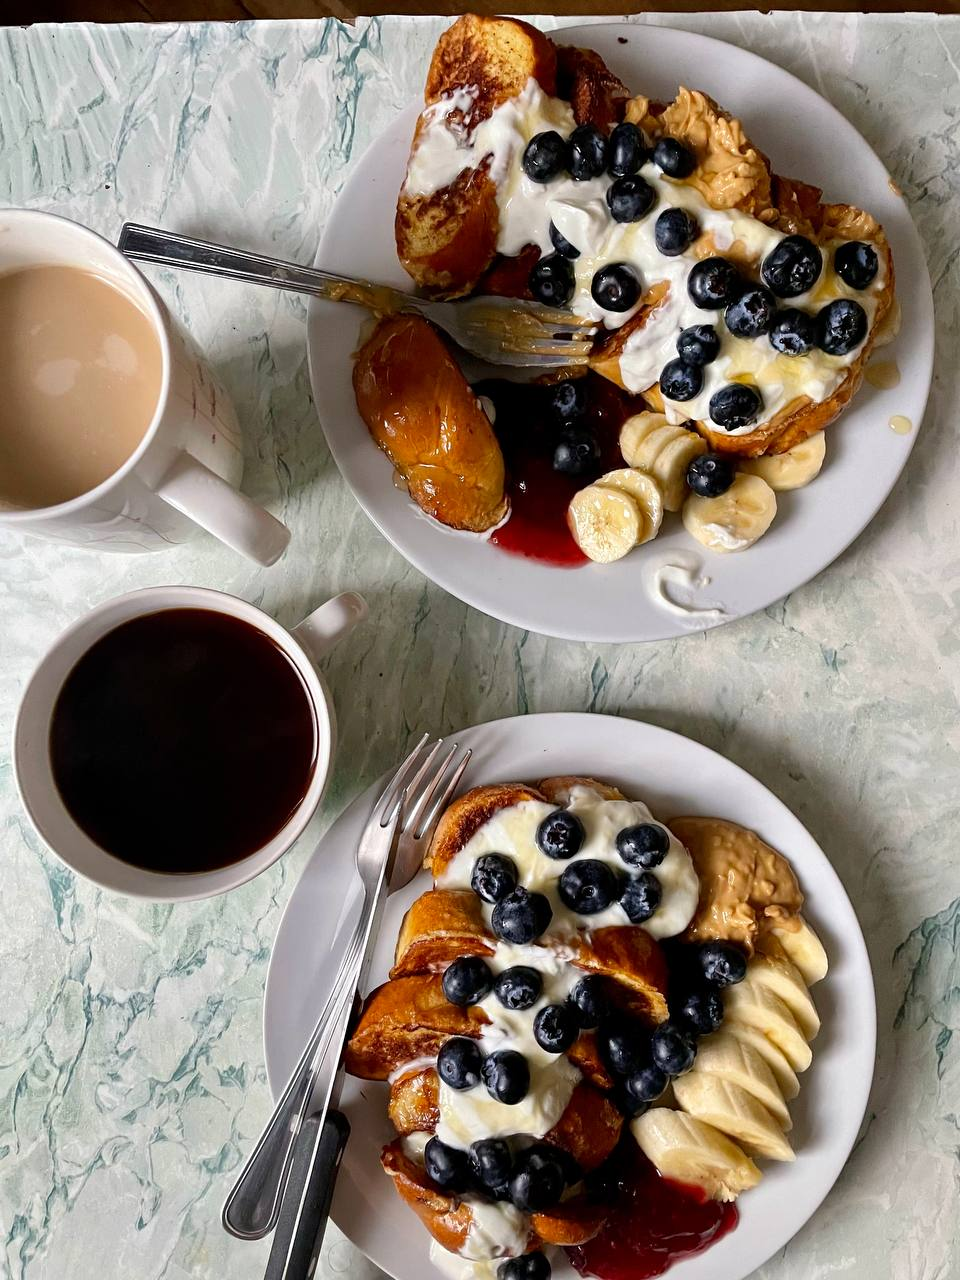
\includegraphics[width=\textwidth]{images/tostynaslodko.jpg}} 
        \caption{Tosty francuskie na słodko}
    \end{minipage}
    
\end{figure}

\newpage

\begin{figure}[H]
    \centering
    \begin{minipage}{0.4\textwidth}
        \centering
        \fbox{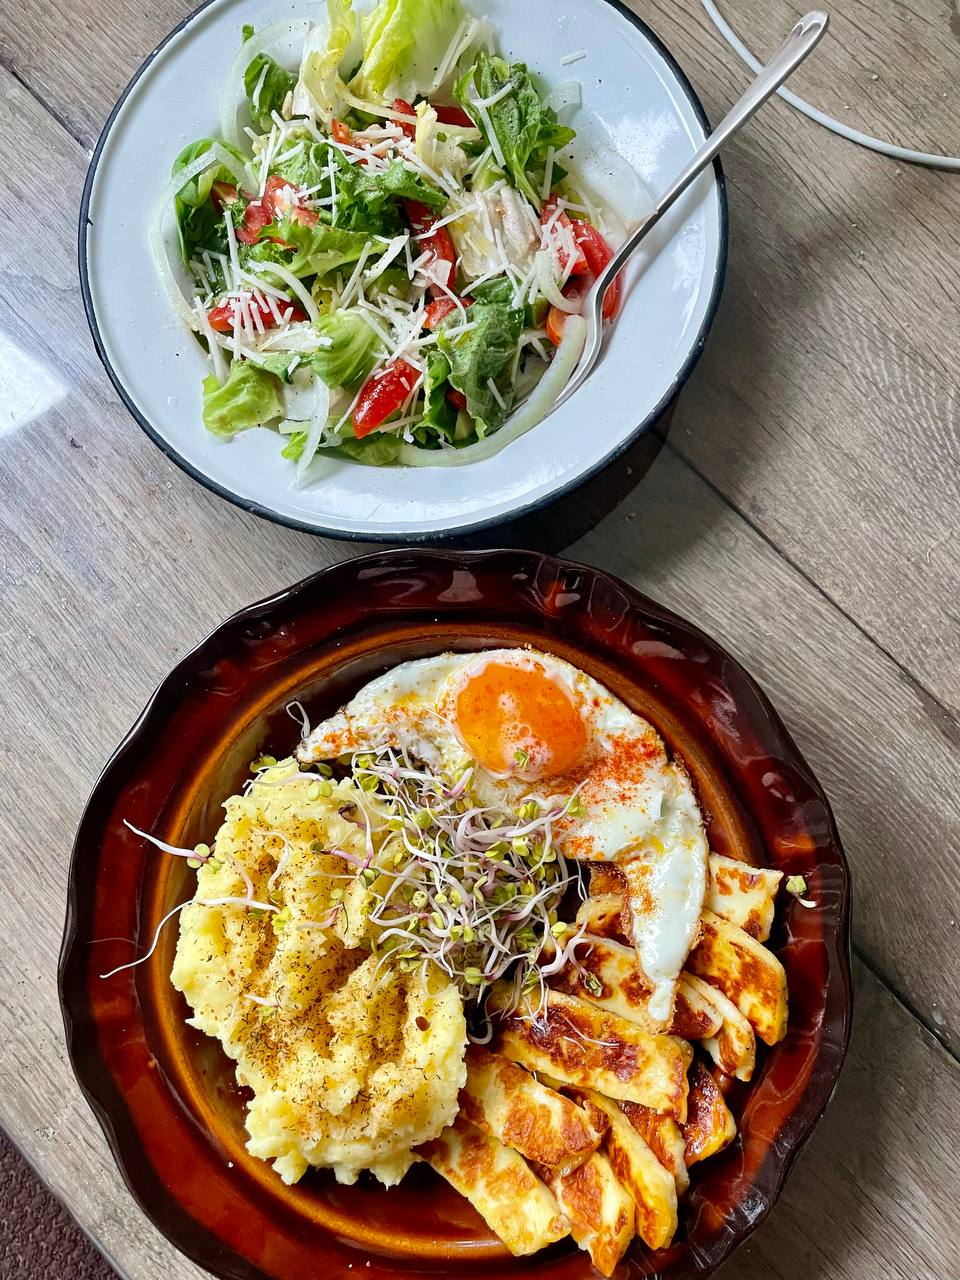
\includegraphics[width=\textwidth]{images/sample10.jpg}} 
        \caption{Puree ziemniaczane ze smażonym serem halloumi, jajkiem i sezonową sałatką}
    \end{minipage}
    \hspace{0.05\textwidth}
    \begin{minipage}{0.4\textwidth}
        \centering
        \fbox{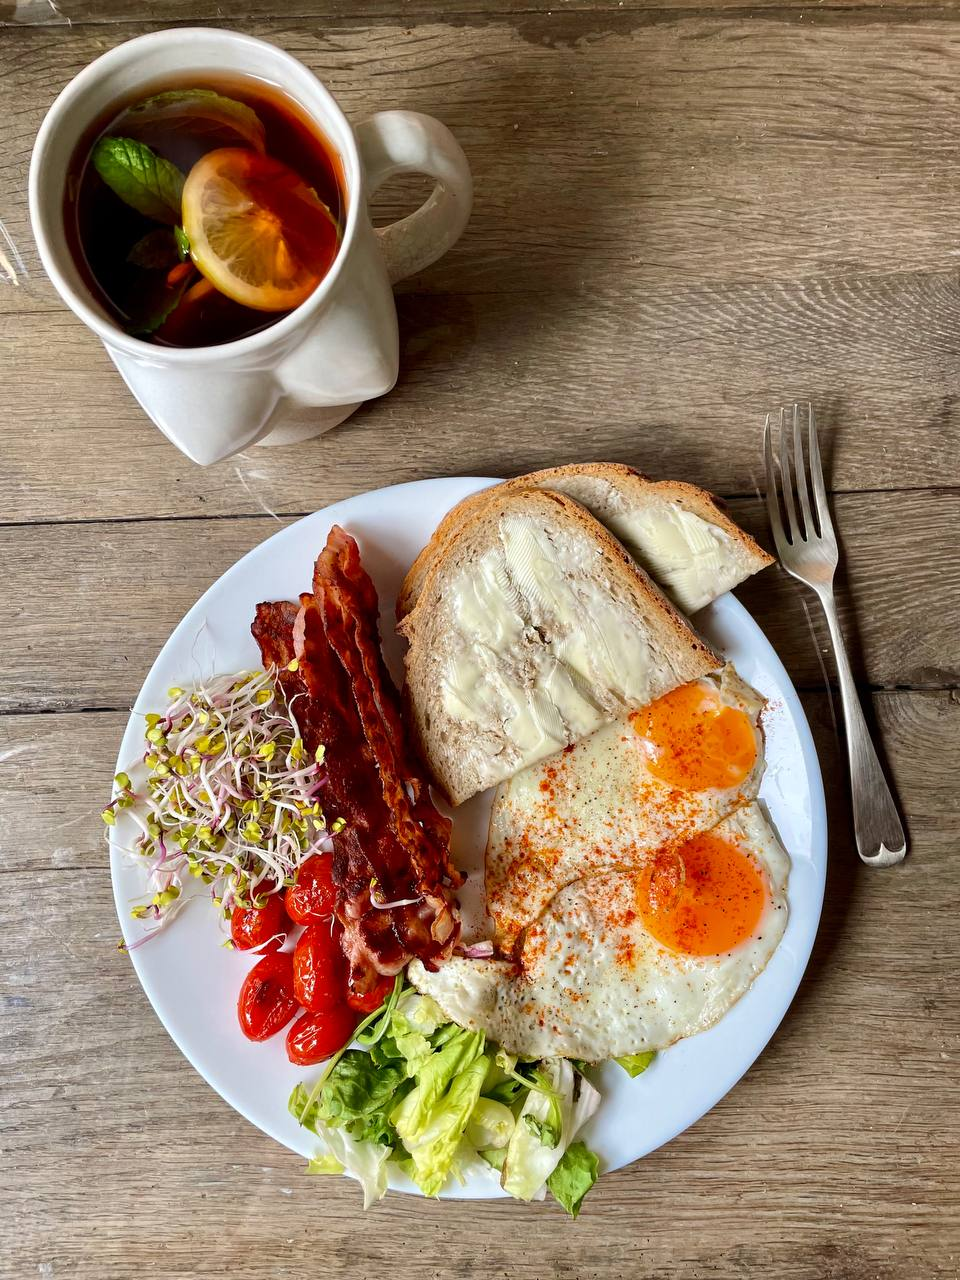
\includegraphics[width=\textwidth]{images/sample8.jpg}}
        \caption{Jajka sadzone z boczkiem i smażonymi pomidorkami}
    \end{minipage}
    
    \vspace{0.05\textwidth}
    
    \begin{minipage}{0.4\textwidth}
        \centering
        \fbox{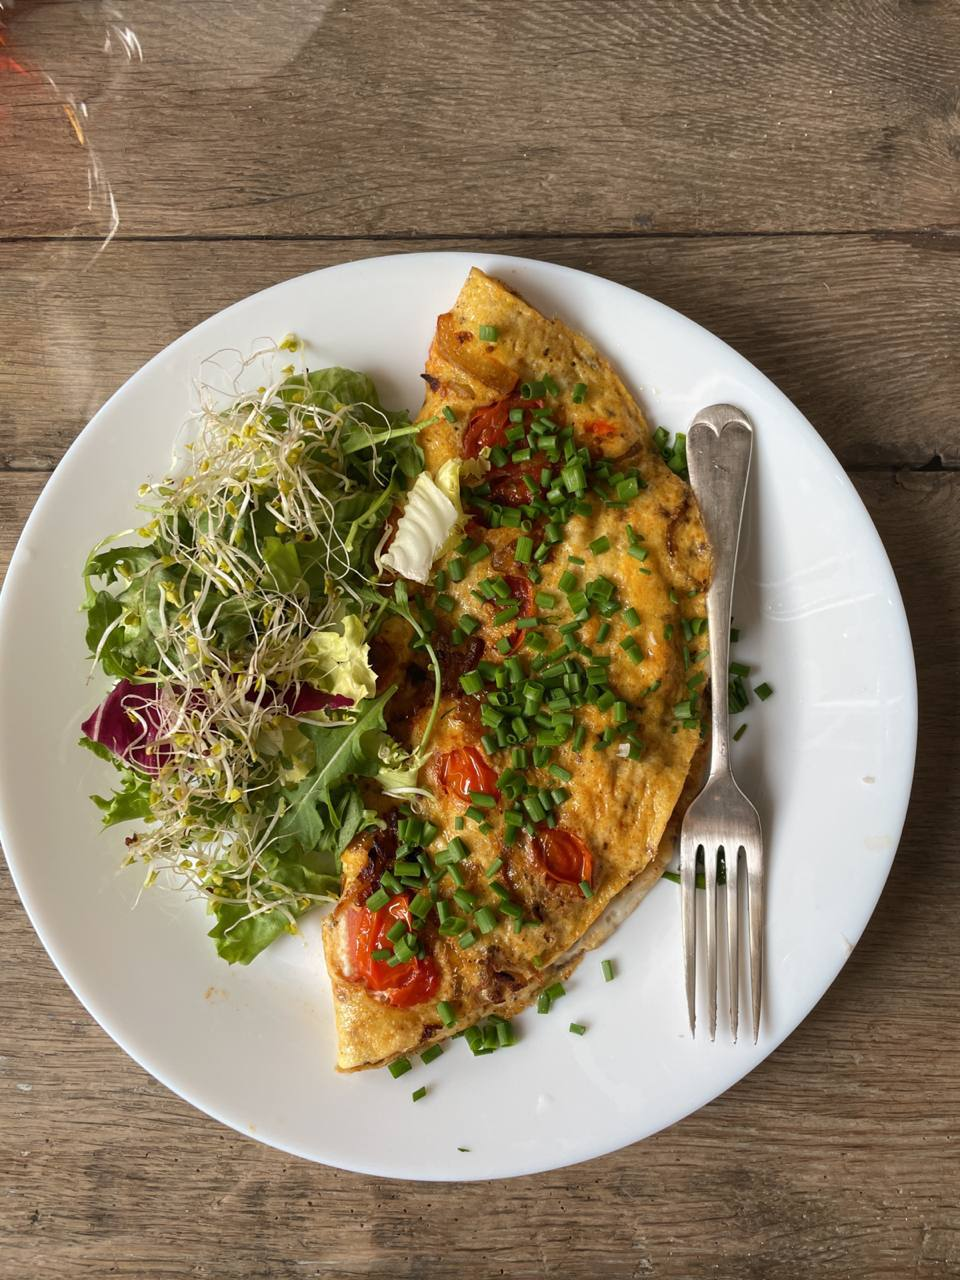
\includegraphics[width=\textwidth]{images/omlet.jpg}} 
        \caption{Omlet z cebulą i pomidorami}
    \end{minipage}
    \hspace{0.05\textwidth} 
    \begin{minipage}{0.4\textwidth}
        \centering
        \fbox{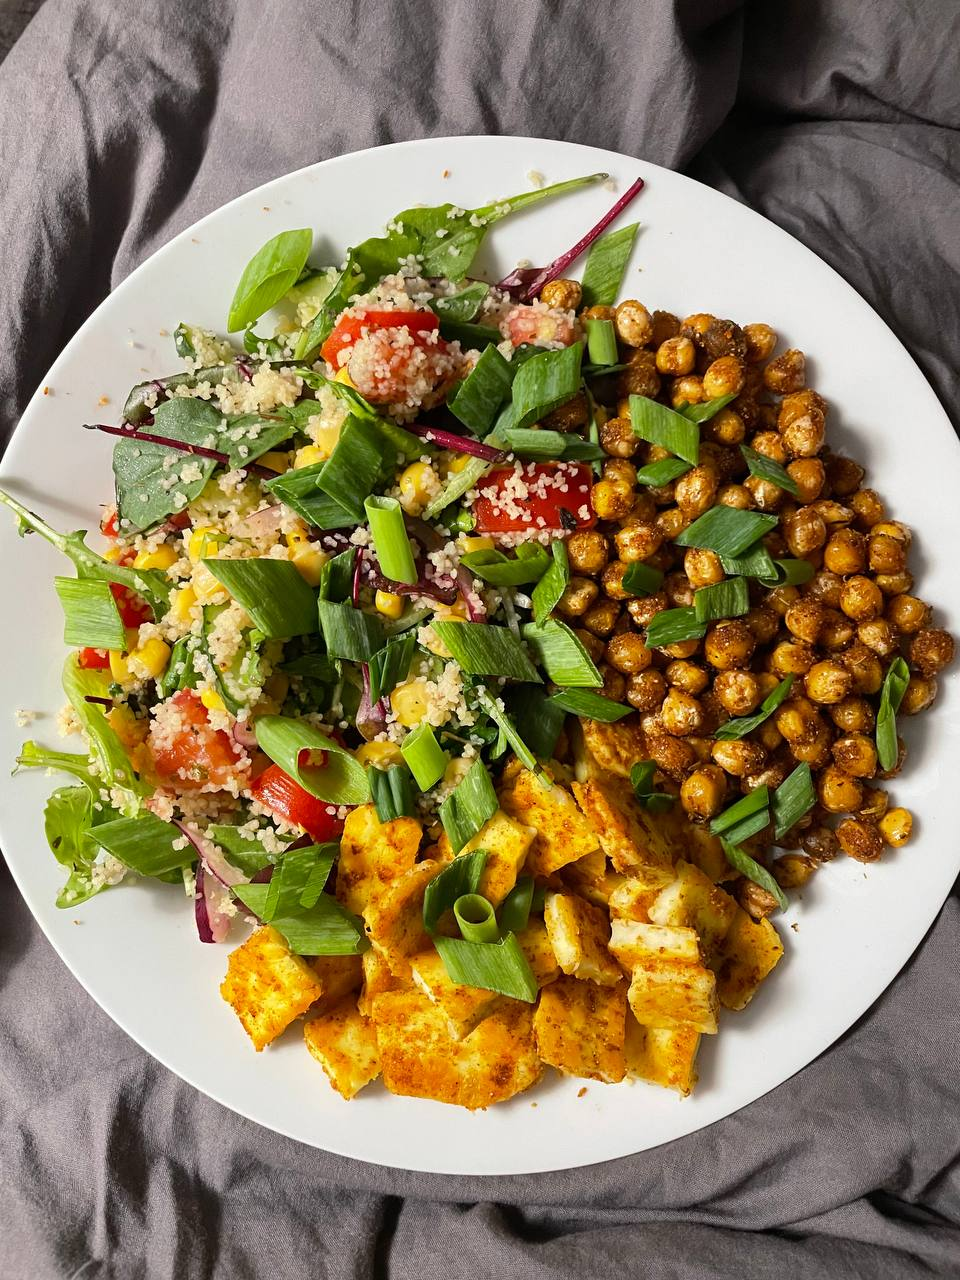
\includegraphics[width=\textwidth]{images/wegebowl.jpg}} 
        \caption{Ciecierzyca pieczona na chrupko ze smażonym serem halloumi i sałatką z kuskusem}
    \end{minipage}
    
\end{figure}

\end{document}

